%% abtex2-modelo-trabalho-academico.tex, v<VERSION> laurocesar
%% Copyright 2012-2015 by abnTeX2 group at http://www.abntex.net.br/ 
%%
%% This work may be distributed and/or modified under the
%% conditions of the LaTeX Project Public License, either version 1.3
%% of this license or (at your option) any later version.
%% The latest version of this license is in
%%   http://www.latex-project.org/lppl.txt
%% and version 1.3 or later is part of all distributions of LaTeX
%% version 2005/12/01 or later.
%%
%% This work has the LPPL maintenance status `maintained'.
%% 
%% The Current Maintainer of this work is the abnTeX2 team, led
%% by Lauro César Araujo. Further information are available on 
%% http://www.abntex.net.br/
%%
%% This work consists of the files abntex2-modelo-trabalho-academico.tex,
%% abntex2-modelo-include-comandos and abntex2-modelo-references.bib
%%

% ------------------------------------------------------------------------
% ------------------------------------------------------------------------
% abnTeX2: Modelo de Trabalho Academico (tese de doutorado, dissertacao de
% mestrado e trabalhos monograficos em geral) em conformidade com 
% ABNT NBR 14724:2011: Informacao e documentacao - Trabalhos academicos -
% Apresentacao
% ------------------------------------------------------------------------
% ------------------------------------------------------------------------

\documentclass[
	% -- opções da classe memoir --
	12pt,				% tamanho da fonte
	openright,			% capítulos começam em pág ímpar (insere página vazia caso preciso)
	%twoside,			% para impressão em verso e anverso. Oposto a oneside
  oneside,     % para impressão em verso e anverso. Oposto a twoside
	a4paper,			% tamanho do papel. 
	% -- opções da classe abntex2 --
	%chapter=TITLE,		% títulos de capítulos convertidos em letras maiúsculas
	%section=TITLE,		% títulos de seções convertidos em letras maiúsculas
	%subsection=TITLE,	% títulos de subseções convertidos em letras maiúsculas
	%subsubsection=TITLE,% títulos de subsubseções convertidos em letras maiúsculas
	% -- opções do pacote babel --
	english,			% idioma adicional para hifenização
	french,				% idioma adicional para hifenização
	spanish,			% idioma adicional para hifenização
	brazil				% o último idioma é o principal do documento
	]{abntex2}

% ---
% Pacotes básicos 
% ---
\usepackage{lmodern}			% Usa a fonte Latin Modern
%\usepackage{cfr-lm}      % Technically, lmodern does since the fonts it installs are identical to those used by cfr-lm		
\usepackage[T1]{fontenc}		% Selecao de codigos de fonte.
\usepackage[utf8]{inputenc}		% Codificacao do documento (conversão automática dos acentos)
\usepackage{lastpage}			% Usado pela Ficha catalográfica
\usepackage{indentfirst}		% Indenta o primeiro parágrafo de cada seção.
\usepackage{color}				% Controle das cores
\usepackage{graphicx}			% Inclusão de gráficos
\usepackage{microtype} 			% para melhorias de justificação

%%%%%%%%%%%%%%%%%%%%%%
% pacotes incluídos
%\usepackage{fontspec}
%\usepackage{fontawesome}
\usepackage{longtable}
\usepackage{lscape}
\usepackage{supertabular}
\usepackage{pdfpages}
\usepackage{hyperref}
\usepackage{courier}
\usepackage{listings}
\usepackage{float}
\definecolor{mygreen}{rgb}{0,0.6,0} \definecolor{mygray}{rgb}{0.5,0.5,0.5} \definecolor{mymauve}{rgb}{0.58,0,0.82}

\lstset{ %
  backgroundcolor=\color{white},   % choose the background color; you must add \usepackage{color} or \usepackage{xcolor}
  basicstyle=\footnotesize\ttfamily,        % the size of the fonts that are used for the code
  breakatwhitespace=false,         % sets if automatic breaks should only happen at whitespace
  breaklines=true,                 % sets automatic line breaking
  captionpos=b,                    % sets the caption-position to bottom
  %commentstyle=\color{mygreen},    % comment style
  deletekeywords={...},            % if you want to delete keywords from the given language
  escapeinside={\%*}{*)},          % if you want to add LaTeX within your code
  extendedchars=true,              % lets you use non-ASCII characters; for 8-bits encodings only, does not work with UTF-8
  frame=single,                    % adds a frame around the code
  keepspaces=true,                 % keeps spaces in text, useful for keeping indentation of code (possibly needs columns=flexible)
  %keywordstyle=\color{blue},       % keyword style
  %language=Octave,                 % the language of the code
  otherkeywords={*,...},            % if you want to add more keywords to the set
  numbers=left,                    % where to put the line-numbers; possible values are (none, left, right)
  numbersep=5pt,                   % how far the line-numbers are from the code
  numberstyle=\tiny\color{mygray}, % the style that is used for the line-numbers
  rulecolor=\color{mygray},         % if not set, the frame-color may be changed on line-breaks within not-black text (e.g. comments (green here))
  showspaces=false,                % show spaces everywhere adding particular underscores; it overrides 'showstringspaces'
  showstringspaces=false,          % underline spaces within strings only
  showtabs=false,                  % show tabs within strings adding particular underscores
  stepnumber=1,                    % the step between two line-numbers. If it's 1, each line will be numbered
  %stringstyle=\color{mymauve},     % string literal style
  tabsize=2,                     % sets default tabsize to 2 spaces
  title=\lstname                   % show the filename of files included with \lstinputlisting; also try caption instead of title
}


%%%%%%%%%%%%%%%%%%%%%%
% ---

% ---
% Pacotes adicionais, usados apenas no âmbito do Modelo Canônico do abnteX2
% ---
\usepackage{lipsum}				% para geração de dummy text
% ---

% ---
% Pacotes de citações
% ---
\usepackage[brazilian,hyperpageref]{backref}	 % Paginas com as citações na bibl
\usepackage[alf]{abntex2cite}	% Citações padrão ABNT

% --- 
% CONFIGURAÇÕES DE PACOTES
% --- 

% ---
% Configurações do pacote backref
% Usado sem a opção hyperpageref de backref
\renewcommand{\backrefpagesname}{Citado na(s) página(s):~}
% Texto padrão antes do número das páginas
\renewcommand{\backref}{}
% Define os textos da citação
\renewcommand*{\backrefalt}[4]{
	\ifcase #1 %
		Nenhuma citação no texto.%
   \or
		Citado na página #2.%
   \else
		Citado #1 vezes nas páginas #2.%
	\fi}%
% ---

% ---
% Configurações de aparência do PDF final

% alterando o aspecto da cor azul
\definecolor{blue}{RGB}{41,5,195}

% definindo comandos para fontawesome

% \newfontfamily{\FA}{FontAwesome Regular}
% \def\twitter{{\FA \faTwitter}}


% informações do PDF
\makeatletter
\hypersetup{
     	%pagebackref=true,
      pdftitle={\@title}, 
      pdfauthor={\@author},
      pdfsubject={\imprimirpreambulo},
      pdfcreator={LaTeX with abnTeX2},
      pdfkeywords={abnt}{latex}{abntex}{abntex2}{trabalho acadêmico}, 
		colorlinks=true,       		% false: boxed links; true: colored links
    	linkcolor=blue,          	% color of internal links
    	citecolor=blue,        		% color of links to bibliography
    	filecolor=magenta,      		% color of file links
      urlcolor=blue,
      bookmarksdepth=4
      }
      \makeatother
% --- 

% --- 
% Espaçamentos entre linhas e parágrafos 
% --- 

% O tamanho do parágrafo é dado por:
\setlength{\parindent}{1.3cm}

% Controle do espaçamento entre um parágrafo e outro:
\setlength{\parskip}{0.2cm}  % tente também \onelineskip

% ---
% compila o indice
% ---
\makeindex
% ---

% ----
% Início do documento
% ----
\begin{document}

%%%%%%%%%%%%%%%%%%%%%%%%%%%%%%%%%%%%%%%%%%%%%%
%%%
%%% Capa e Contra-Capa
%%%
%%%%%%%%%%%%%%%%%%%%%%%%%%%%%%%%%%%%%%%%%%%%%%


\begin{center} 

\includegraphics[scale=0.25]{images/ufpelogo.pdf} \\

{\scshape Universidade Federal de Pernambuco\\}
{\scshape Centro de Tecnologia e Geociências\\}
{\scshape Programa de Pós-Graduação em Engenharia Elétrica\\}
%{\scshape Circuitos Integrados e Sistemas Embarcados\\}
\vfill
        %\vspace{4.5cm}
        {{\Large \textbf{Circuitos Integrados e Sistemas Embarcados}}}\\
        \vspace{.5cm}
        {{\Large Relatório Final}}\\
        \vspace{1cm}
        {{\large Versão: 1.0.0}}\\
        \vfill

        Universidade Federal de Pernambuco\\
        Centro de Tecnologia e Geociências/Escola de Engenharia\\
        Programa de Pós-Graduação em Engenharia Elétrica\\
        Departamento de Eletrônica e Sistemas - Bloco B, 4º andar, sala 416.\\

        Avenida da Arquitetura, s/n -- Cidade Universitária\\
        50740-550 - Recife - Pernambuco - Brasil\\

        Fone: +55 81 2126-7117 --- Fax: +55 81 2126-8215

        \url{https://www.ufpe.br/ppgee}\\ \vskip\baselineskip

        \vspace{0.5cm}
        \vskip\baselineskip
        Recife, 27 de julho de 2015
        \end{center}



\newpage


%%%%%%%%%%%%%%%%%%%%%%%%%%%%%%%%%%%%%%%%%%%%%%%%%%%%%%%%
%%%
%%% Dados da Criação/Autorização/Reconhecimento do Curso
%%%
%%%%%%%%%%%%%%%%%%%%%%%%%%%%%%%%%%%%%%%%%%%%%%%%%%%%%%%%

\chapter*[Licença deste conteúdo]{Licença deste conteúdo}
\addcontentsline{toc}{chapter}{Licença deste conteúdo}

Com o objetivo de promovermos ampla divulgação e possibilitar a participação ativa (de professores, estudantes, egressos, profissionais e da comunidade em geral) no desenvolvimento e aprendizagem da área de Circuitos Integrados e Sistemas Embarcados, disponibilizamos este Relatório Final de Disciplina no Repositório GitHub.

\vfill

\begin{figure}[ht]
  \centering
  
\includegraphics[width=0.3\textwidth]{images/by-nc-sa.jpg}
\end{figure}

\noindent Circuitos Integrados e Sistemas Embarcados - Relatório Final de Gustavo Esteves, João Ferreira, Kádna Maria e Sérgio Mendonça está licenciado com uma Licença Creative Commons --  Atribuição (BY) -- Não Comercial (NC) -- Compartilha Igual (SA) 4.0 Internacional. Baseado no trabalho disponível em \url{https://github.com/sftom/ee1054}.

\hfill \noindent A equipe.

\newpage

%%%%%%%%%%%%%%%%%%%%%%%%%%%%%%%%%%%%%%%%%%%%%%%%%%%%%%%%
%%%
%%% Comissão de Elaboração da Reforma Curricular do Curso
%%%
%%%%%%%%%%%%%%%%%%%%%%%%%%%%%%%%%%%%%%%%%%%%%%%%%%%%%%%%

\chapter*[Equipe de Elaboração e \\Resolução das Atividades]{Equipe de Elaboração e \\Resolução das Atividades}
\addcontentsline{toc}{chapter}{Equipe de Elaboração e Resolução das Atividades}


\section*{Elaboração das Atividades}

\noindent Prof. Marco Aurélio Benedetti Rodrigues\\
\url{http://lattes.cnpq.br/2448324832915432}\\



\section*{Estudantes --- Execução das Atividades}

\noindent Gustavo Ribeiro Porpino Esteves\\
\url{http://lattes.cnpq.br/1140864652601909}\\

\noindent João Ferreira da Silva Júnior\\
\url{http://lattes.cnpq.br/8904695743376784}\\

\noindent Kádna Marina Alves Camboim Vale\\
\url{http://lattes.cnpq.br/2817387497612302}\\

\noindent Sérgio Francisco Tavares de Oliveira Mendonça\\
\url{http://lattes.cnpq.br/6313698968060384}\\

\newpage

% Seleciona o idioma do documento (conforme pacotes do babel)
%\selectlanguage{english}
\selectlanguage{brazil}

% Retira espaço extra obsoleto entre as frases.
\frenchspacing 

% ---
% inserir lista de ilustrações
% ---
\pdfbookmark[0]{\listfigurename}{lof}
\listoffigures*
\cleardoublepage
% ---

% ---
% inserir lista de tabelas
% ---
\pdfbookmark[0]{\listtablename}{lot}
\listoftables*
\cleardoublepage
% ---

% ---
% inserir lista de abreviaturas e siglas
% ---
\begin{siglas}
\item[UFPE] Universidade Federal de Pernambuco
\item[PPGEE] Programa de Pós-Graduação em Engenharia Elétrica
\item[CTG] Centro de Tecnologia e Geociências
\end{siglas}
% ---

% ---
% inserir lista de símbolos
% ---
% \begin{simbolos}
%   \item[$ \Gamma $] Letra grega Gama
%   \item[$ \Lambda $] Lambda
%   \item[$ \zeta $] Letra grega minúscula zeta
%   \item[$ \in $] Pertence
% \end{simbolos}
% ---

% ---
% inserir o sumario
% ---
\pdfbookmark[0]{\contentsname}{toc}
\tableofcontents*
\cleardoublepage
% ---



% ----------------------------------------------------------
% ELEMENTOS TEXTUAIS
% ----------------------------------------------------------
\textual

% ----------------------------------------------------------
% Introdução (exemplo de capítulo sem numeração, mas presente no Sumário)
% ----------------------------------------------------------
\chapter*[Introdução]{Introdução}
\addcontentsline{toc}{chapter}{Introdução}
% ----------------------------------------------------------

\section*{A área de Circuitos Integrados e Sistemas Embarcados}

De acordo com o atual crescimento tecnológico, pode-se estimar que a era da Internet das Coisas, do Inglês, \textit{Internet of Things} (IoT) demandará por bilhões de novos dispositivos nos próximos 5 anos. Este cenário aponta uma crescente demanda por equipamentos que consumam menos energia, ou que esta seja uma fonte renovável, que executem a transmissão de dados em tempo-real, que disponha de estratégias otimizadas para a manipulação de algoritmos ou de dados, entre outros aspectos. Sem falar da necessidade dos sistemas que interagem uns com os outros.

% section introdução_ (end)

\section*{Requisitos para Sistemas Embarcados} % (fold)
\label{sec:requisitos}

Ao iniciar qualquer projeto, é preciso levantar uma série de questões que possibilitem um melhor entendimento das necessidades, questionar pontos que se mostrem relevantes, e verificar se há concorrência com projetos semelhantes, bem como nos aprofundar nos pontos principais das especificações desejadas.

Uma declaração de escopo precisa ser definida, contendo características principais do sistema, restrições (técnicas, financeiras, comerciais, de tecnologia...), estamos falando especificamente dos requisitos do produto, que envolvem requisitos de hardware e de software (este já pode conter muitas bibliotecas disponíveis, além de entendimentos concisos).

É preciso entender que os requisitos nem sempre são muitos bem especificados, muitas vezes por pouca maturidade no desenvolvimento, por parte do desenvolvedor, muitas vezes por falta da adoção de técnicas ou de uma abordagem sistemática no levantamento desses requisitos.

Independentemente dos caminhos que um projeto venha a tomar, tem-se dois grandes grupos de preocupações:

\begin{itemize}
    \item O que o sistema deve fazer?
    \item E, como ele deve implementar todos os requisitos?
\end{itemize}

A disciplina de Circuitos Integrados e Sistemas Embarcados tem como ementa a análise e projetos com circuitos integrados analógicos e digitais utilizados em instrumentação eletrônica, possibilitando o desenvolvimento de aplicações, utilizando microcontroladores em sistemas embarcados e circuitos de tempo real. Assim, é possível encontrar as respostas às questões citadas acima, quando se tratando do projeto da disciplina, quanto para projetos de âmbito mercadológico.

\section*{Organização deste Relatório} % (fold)
\label{sec:organizacao_deste_relatorio}

Este relatório final apresenta as atividades realizadas ao longo da Disciplina de Circuitos Integrados e Sistemas Embarcados. Foram desenvolvidas oito atividades, cada uma com propósito específico para determinado tipo de microcontrolador ou placa. Para cada atividade são apresentadas as questões propostas, a resolução de cada uma delas, bem como os códigos em linguagem de programação e algumas considerações. O presente relatório está organizado da seguinte forma: a atividade 1 trata do microcontrolador MCS51, a atividade 2 é sobre o microcontrolador Atmel AT89S51, a atividade 3 apresenta o microcontrolador PIC, a atividade 4 vem com o microcontrolador MSP-430, na atividade 5 temos o microcontrolador MSP430-GRACE, na atividade 6 é apresentado o microcontrolador Kinetis Freescale, já nas atividades 7 e 8 são apresentadas as placas Raspberry Pi B+ e Intel Galileo, respectivamente.

Com o objetivo de colaborar com a comunidade, também disponibilizamos todo o material desenvolvido no GitHub.com, disponível em \url{https://github.com/sftom/ee1054}, para que estes possam servir de orientações e desenvolvimento de estudantes e profissionais da área.

% section organizacao_deste_relatorio (end)

%%%%%%%%%%%%%%%%%%%%%%%%%%%%%%%%%%%%%%%%%%%%%%%%%%%%%%%%%%%%%%%%%%%%%%%%%%%%%%%%%%%%%
%
% chapter: Trabalho I - Família MCS51
%
%%%%%%%%%%%%%%%%%%%%%%%%%%%%%%%%%%%%%%%%%%%%%%%%%%%%%%%%%%%%%%%%%%%%%%%%%%%%%%%%%%%%%%

\chapter{Microcontrolador MCS51} % (fold)
\label{cha:1-Familia-MCS51}

\section{Atividades propostas} % (fold)
\label{sec:atividades_propostas}

\subsection*{Trabalho I – Aula teórica com microcontrolador família MCS51}

\subsubsection*{Atividade 1}

\noindent Baseado no circuito abaixo realizar o que se pede:

\begin{enumerate}
  \item Identificar a função do circuito e explicar a função dos componentes eletrônicos utilizados no projeto.
  \item Quantos canais estão sendo convertidos para o domínio digital? Proponha o circuito para a utilização dos demais canais do ADC0808.
  \item Qual a taxa de amostragem do conversor A/D e quantização utilizada no circuito. Explique.
  \item Qual a máxima velocidade permitida para a conversão A/D desse circuito? O que deve ser feito para atingir essa velocidade?
  \item E em função do grau de quantização, isto é, da resolução do sinal de tensão convertido, o que se pode fazer para melhorar a qualidade do sinal digital?
  \item Faça um programa em C, com a finalidade de:
  \begin{enumerate}
    \item Controlar o A/D do circuito conforme o esquemático;
    \item Controlar o A/D para a utilização total dos canais.
  \end{enumerate}
\end{enumerate}

\begin{figure}[ht]
  \centering
  \caption{\label{fig:Atividade-01-esquematico.png}Diagrama Esquemático da Família MCS51 utilizado na Atividade~\ref{cha:1-Familia-MCS51}.}
  \fonte{Produzido pelo Prof. Marco Aurélio Benedetti Rodrigues}
  \includegraphics[width=0.8\textwidth]{images/Atividade01/Atividade-01-esquematico.png}
\end{figure}
% section atividades_propostas (end)

\section{Relatório da Atividade} % (fold)
\label{sec:consideracoes-cap-1}

\noindent As atividades acima são respondidas a seguir:

\begin{enumerate}
  \item O circuito recebe um sinal analógico a partir do LM324 que amplifica esse sinal e o envia para a entrada IN3 do ADC0808, que faz a amostragem do sinal convertendo de analógico para digital e enviando para o microcontrolador AT89C51, que exibe o sinal amostrado no display 16X21CD, ou seja, recebe o sinal analógico, converte para digital e exibe no LCD.
  \item Apenas um sinal está sendo convertido para o domínio digital IN3 do ADC0808. A proposta para o circuito é replicar o circuito de aquisição do LM324 para cada uma das portas disponíveis do conversor A/D (IN4, IN5, IN6, IN7, IN2, IN1 e IN0) e em seguida considerar a informação dos pinos de endereçamento (ADDR\_A, ADDR\_B e ADDR\_C) que informa qual a porta de entrada do sinal analógico junto com a informação da porta ALE, que sinaliza a finalização do endereço novo.
  \item A taxa de amostragem do conversor A/D é 10khz, pois seu tempo de conversão é de 100 microssegundos. Mas, como o circuito A/D utiliza apenas uma porta e possui o clock de 687khz, a taxa de amostragem será de 10,735khz. A quantização utilizada no circuito é de 8 bits, o que dá 255 níveis.
  \item A velocidade máxima permitida se obtém elevando-se o clock para 1280khz e curto-circuitar os pinos SC e EOC do conversor A/D, o que já está feito no circuito.
  \item Para melhorar a qualidade do sinal digital deve-se ajustar os limites de saída do LM324 de acordo com os limites de entrada do ADC0808.
  \item A descrição do fluxo do programa pode ser observado a seguir, bem como um pseudocódigo, desenvolvido em Linguagem C.
  \begin{enumerate}
    \item O MC envia o endereço a ser lido pelas portas  ADDR\_A, ADDR\_B e ADDR\_C, com o valor de A=0, B=1 e C=1 que corresponde a porta ANALOG\_IN3 do conversor A/D. Após isso, aciona o latch em nível alto, dá um delay de 200 ms  para aguardar a conversão pelo A/D e aciona o pino OE para habilitar a leitura do valor de saída, executa a leitura. Os pinos SC e EOC não são controlados, pois, estão curto-circuitados.
    \item O MC envia o endereço a ser lido pelas portas ADDR\_A, ADDR\_B e ADDR\_C com seus valores variando de 000 até 111, correspondendo às portas ANALOG\_IN[0-7] do conversor A/D, para cada endereço repete-se o seguinte processo: aciona o latch em nível alto, dá um delay de 200ms e enviar o latch  (ALE), para o nível baixo, novamente da outro delay de 200ms para aguardar a conversão A/D e aciona o pino OE para habilitar a leitura do valor de saída, executa a leitura. A partir daqui segue para o próximo endereço ANALOG\_IN, do início desse processo. Os pinos SC e EOC não são controlados, pois estão curto-circuitados. 
  \end{enumerate}
\end{enumerate}

Para fonte de consulta, inserimos o Diagrama de Bloco, como pode ser observado na Figura~\ref{fig:datasheet-cap1-2}, extraída do Data Sheet do MCS51. \cite{Corporation2000}.

Podemos observar um fluxo do programa na Figura~\ref{fig:cha-1-fluxograma}, com a ideia de melhorar o entendimento do programa, e a partir deste, construir o código em Linguagem C.

\begin{figure}[H]
  \centering  
  \caption{\label{fig:cha-1-fluxograma}Fluxograma do controle A/D do circuito para utilização total dos canais.}
  \fonte{Produzido pelos autores.}
  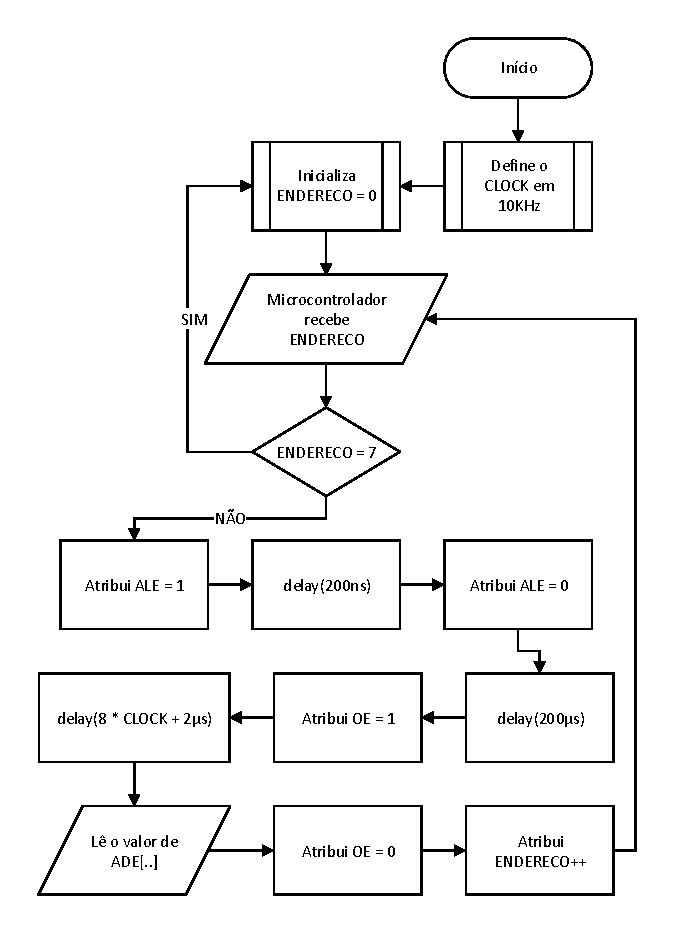
\includegraphics[width=0.7\textwidth]{images/Atividade01/Fluxograma.pdf}
\end{figure}

\newpage
%inserindo algumas páginas: 1 até 7, depois 50 e 57

  \begin{figure}[H]
    \centering
    \includepdf[pages=2,frame=true,width=0.9\textwidth,pagecommand={}]{datasheets/A4-A1-A2-doc0265.pdf}
    \caption{\label{fig:datasheet-cap1-2}Diagrama de Bloco do Data Sheet do MCS51}
  \end{figure}

\newpage

Os pseudocódigos elaborados estão disponibilizados a seguir:

\section*{Microcontrolador MCS51 80C51 -- A01 (Pseudocódigo)}
\subsection*{A01Q06a}
\lstinputlisting{sources/EE1054-Atividade01-6A.alg}

\subsection*{A01Q06b}
\lstinputlisting{sources/EE1054-Atividade01-6B.alg}

% section considerações (end)

% chapter cha:Trab-1-Familia-MCS51 (end)

















%%%%%%%%%%%%%%%%%%%%%%%%%%%%%%%%%%%%%%%%%%%%%%%%%%%%%%%%%%%%%%%%%%%%%%%%%%%%%%%%%%%%%
%
% chapter 2: Microcontrolador ATMEL AT89S51
%
%%%%%%%%%%%%%%%%%%%%%%%%%%%%%%%%%%%%%%%%%%%%%%%%%%%%%%%%%%%%%%%%%%%%%%%%%%%%%%%%%%%%%%

\chapter{Microcontrolador ATMEL AT89S51}% (fold)
\label{cha:2-ATMEL-AT89S51}

\section{Atividades propostas} % (fold)
\label{sec:atividades_propostas-AT89S51}

\subsection*{Relatório de experimentos – Aula prática com microcontrolador família MCS51}

\subsubsection*{Atividade 2}

\begin{enumerate}
\item Desenvolver um programa para realizar as seguintes funções:
\begin{enumerate}
\item Ao pressionar uma tecla acender e apagar todos os quatro LEDs da placa.
\item Ao pressionar a segunda tecla fazer com que os quatro LEDs se acendam em ordem crescente.
\item Ao pressionar a terceira tecla fazer com que os quatro LEDs se acendam em ordem decrescente.
\item Ao pressionar a quarta tecla realizar o item a, b e c em sequência.
\end{enumerate}
\end{enumerate}

% section atividades_propostas (end)

\section{Relatório da Atividades} % (fold)
\label{sec:Consideracoes-AT89S51}

A seguir, podemos visualizar uma imagem do microcontrolador MCS51 utilizado para a realização dos experimentos.

\begin{figure}[ht]
  \centering
  \caption{\label{fig:Microcontrolador-KL-Intel-P8051}Microcontrolador KL Intel P8051.}  
  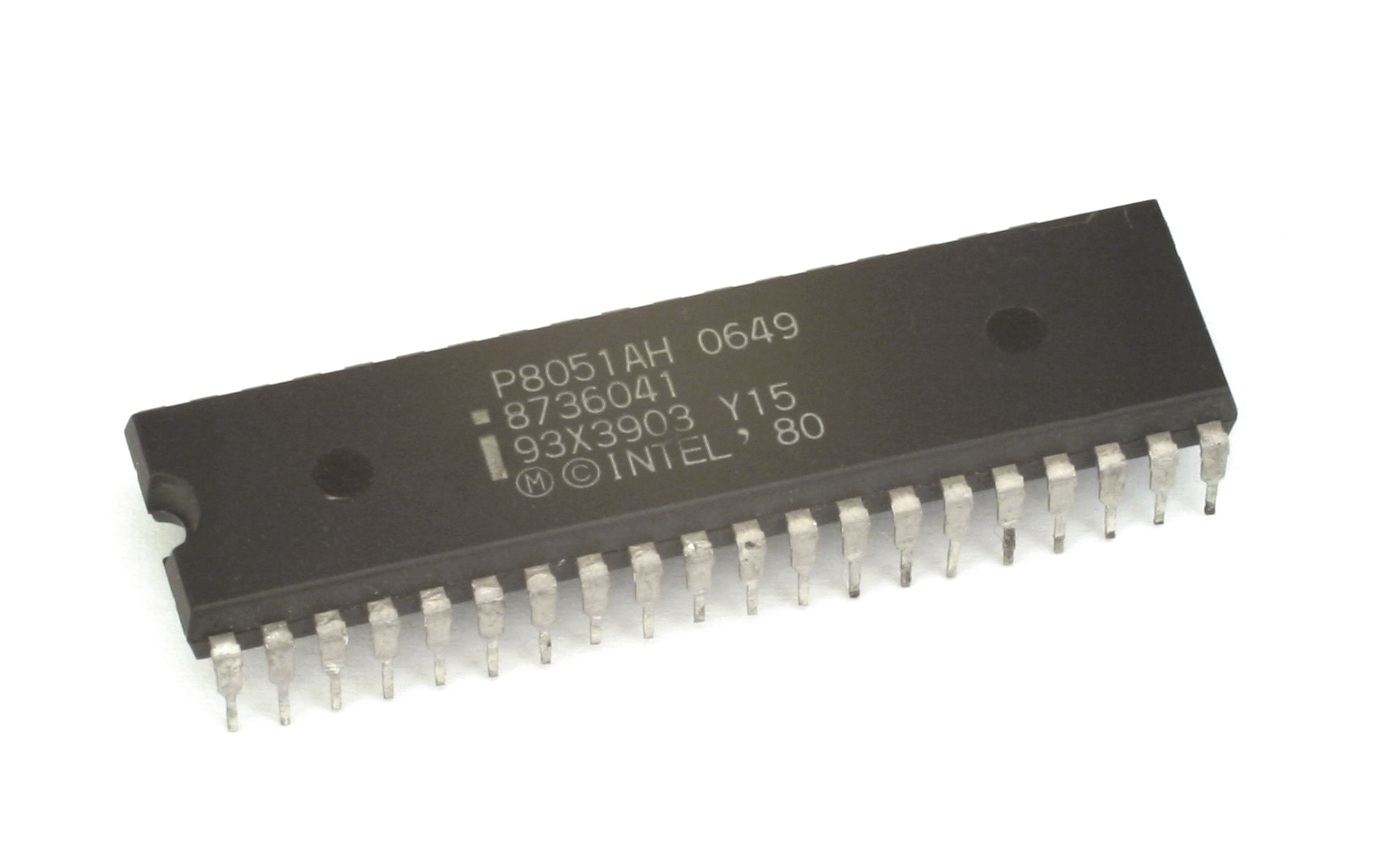
\includegraphics[width=0.4\textwidth]{images/Atividade02/Atividade-02-03-Microcontrolador-KL_Intel_P8051.jpg}
\end{figure}

Para essa atividade foi utilizado o Reads51 que permite simular as entradas e saídas do controlador través de botões mostrados na Figura~\ref{fig:Reads51-teste-C}.

\begin{figure}[ht]
  \centering  
  \caption{\label{fig:Reads51-teste-C}Executando código em simulador para embarcados Reads51.} 
  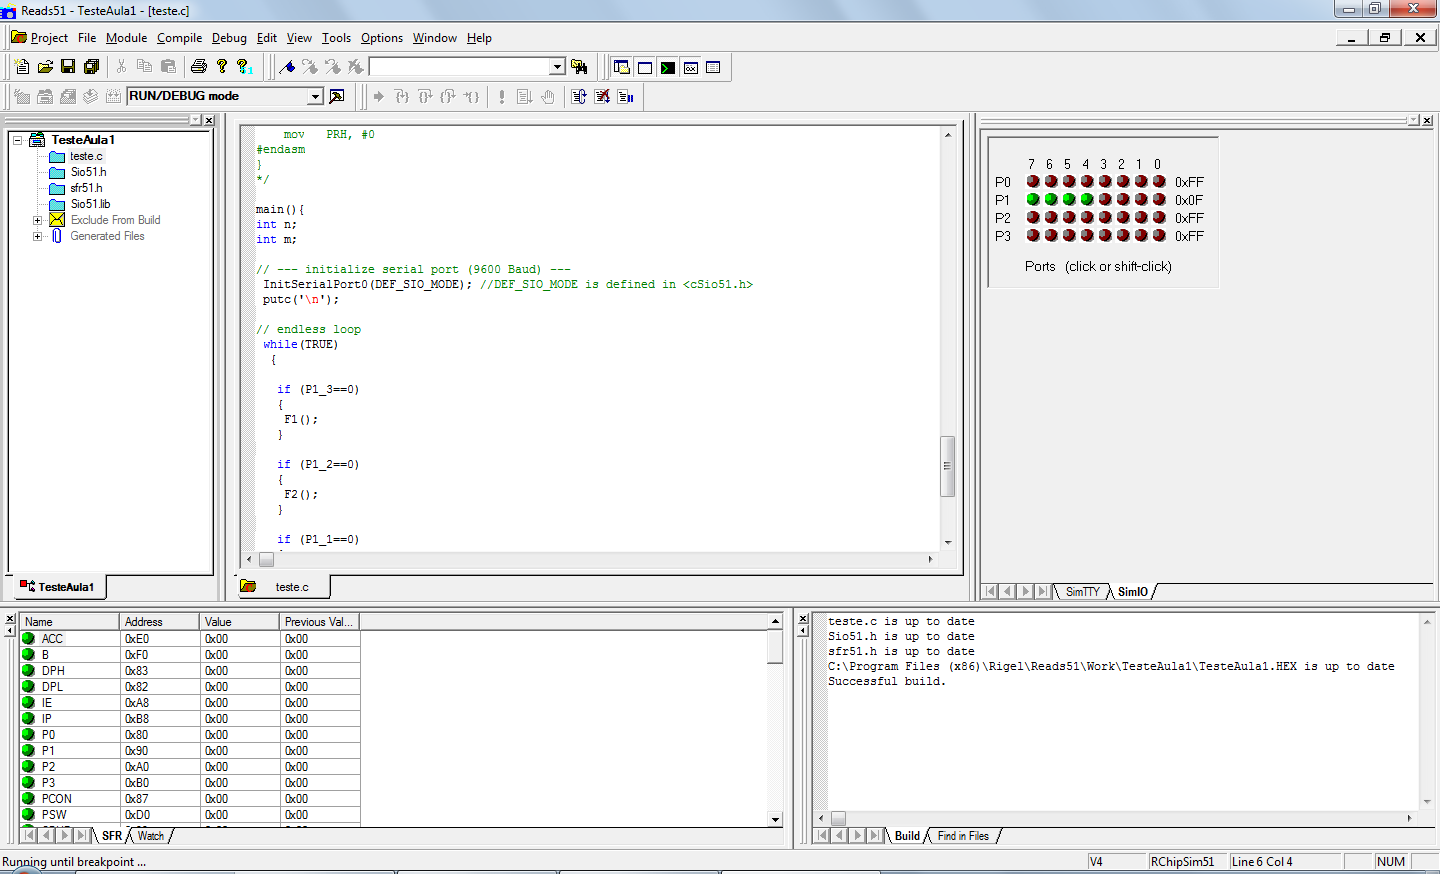
\includegraphics[width=0.9\textwidth]{images/Atividade02/Atividade-02-02-Reads51-teste-c.png} 
\end{figure}

A gravação dos códigos desenvolvidos no MCS51 é realizada através de um gravador, como mostrado na Figura~\ref{fig:Gravador-Firmware-MCS51}.

\begin{figure}[ht]
  \centering
  \caption{\label{fig:Gravador-Firmware-MCS51}Gravador de firmware para Microcontrolador MCS51.}
  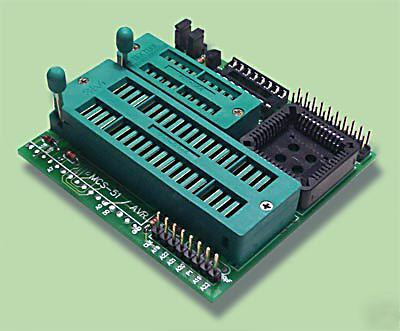
\includegraphics[width=0.6\textwidth]{images/Atividade02/Atividade-02-04-Gravador-MCS-51.jpg}
\end{figure}

\begin{figure}[ht]
  \centering
  \caption{\label{fig:Atividade-02-05-Schematic-01}Diagrama Esquemático desenvolvido para o MCS51 80C51 durante a Atividade~\ref{cha:2-ATMEL-AT89S51}.}
  \fonte{Produzido pelos autores.}
  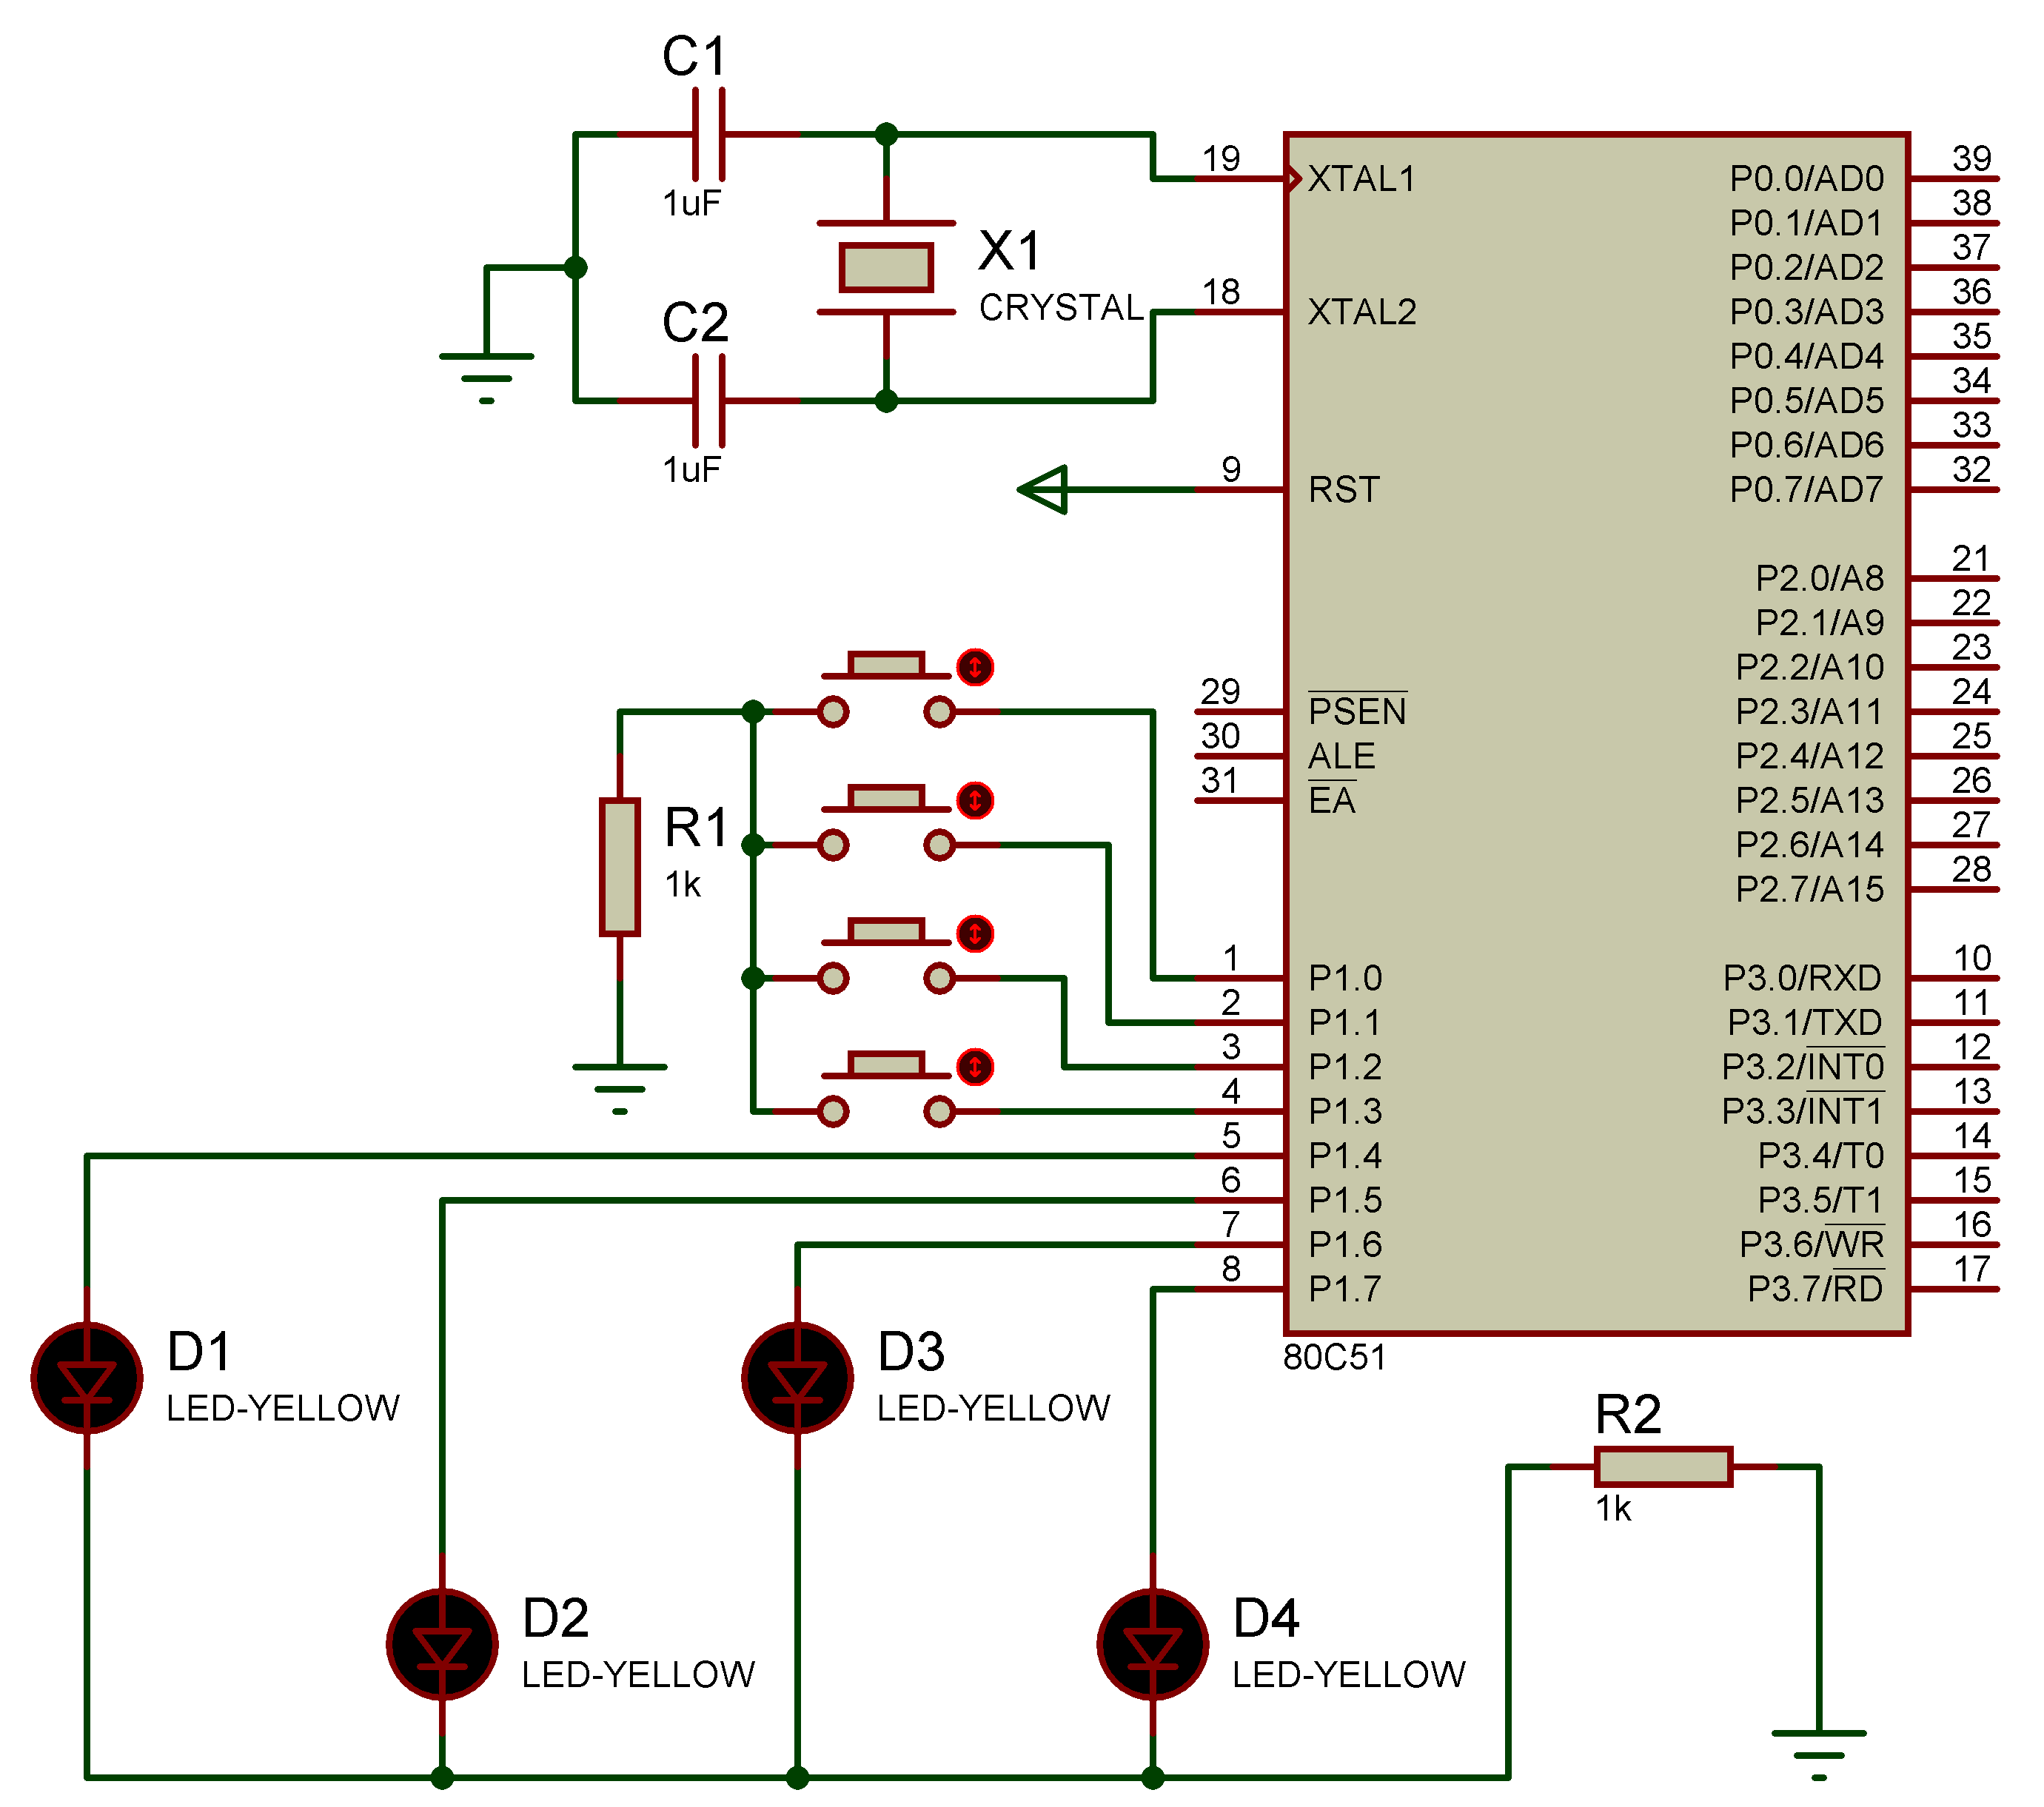
\includegraphics[width=0.8\textwidth]{images/Atividade02/Atividade-02-05-Schematic-01.png}  
\end{figure}

Conforme solicitado na Atividade~\ref{cha:2-ATMEL-AT89S51} foi necessária a utilização de uma placa de circuito cedida para as equipes, que continha os componenetes que seria utilizados, como por exemplo, botões e LED's. O Diagrama Esquemático das ligações realizadas na placa pode ser observado na Figura~\ref{fig:Atividade-02-05-Schematic-01}.



Como trabalhamos, teoricamente, no mesmo microcontrolador da Atividade~\ref{cha:1-Familia-MCS51}, inserimos novamente o Diagrama de Bloco, como pode ser observado na Figura~\ref{fig:datasheet-cap1-2}, extraída do Data Sheet do Atmel AT89S51. \cite{Corporation2000}.

\newpage
%inserindo algumas páginas: 1 até 7, depois 50 e 57

  \begin{figure}[H]
    \centering
    \includepdf[pages=2,frame=true,width=0.9\textwidth,pagecommand={}]{datasheets/A4-A1-A2-doc0265.pdf}
    \caption{\label{fig:datasheet-cap1-2-2}Diagrama de Bloco do Data Sheet do MCS51.}
  \end{figure}

\newpage

Os códigos-fontes elaborados estão disponibilizados a seguir:

\section*{Microcontrolador ATMEL AT89S51 -- A02 (Códigos-fontes)}
\subsection*{A02Q01}

\lstinputlisting{sources/EE1054-Atividade02.c}

% section considerações_finais (end)

% chapter ATMEL-AT89S51 (end)















%%%%%%%%%%%%%%%%%%%%%%%%%%%%%%%%%%%%%%%%%%%%%%%%%%%%%%%%%%%%%%%%%%%%%%%%%%%%%%%%%%%%%
%
% chapter 3: Microcontrolador PIC
%
%%%%%%%%%%%%%%%%%%%%%%%%%%%%%%%%%%%%%%%%%%%%%%%%%%%%%%%%%%%%%%%%%%%%%%%%%%%%%%%%%%%%%%

\chapter{Microcontrolador PIC18F4550}% (fold)
\label{cha:3-PIC}

\section{Atividades propostas} % (fold)
\label{cha:PIC-sec:atividades_propostas}

\subsection*{Relatório de experimentos – Aula prática com microcontrolador família PIC}

\subsubsection*{Atividade 3}

\begin{enumerate}
  \item Instalar o programa para bootloader e o simulador cruzado MicroC: InstallPROTOn e microc-pro-pic640. 
  \item Fazer um programa para acionar dois LEDs da placa PIC fornecida. Utilizar o arquivo Manual PROTOn para identificar os LEDs e onde estão conectados.
  \item Ao pressionar uma tecla, acender e depois apagar todos os dois LEDs da placa.
  \item Ao pressionar pela segunda vez a tecla, fazer com que os 2 LEDs se acendam da seguinte forma:
  \begin{enumerate}
    \item LED 1 acende e apaga a cada 100ms
    \item Após 10 piscadas do LED1 o LED2 fica aceso por 100ms.
  \end{enumerate}
\end{enumerate}

% section atividades_propostas (end)

\section{Relatório da Atividade} % (fold)
\label{sec:consideracoes-PIC}

\begin{figure}[ht]
  \centering
  \caption{\label{fig:03MicrocontrollerPIC_18F4550}Microcontrolador PIC18F4550.} 
  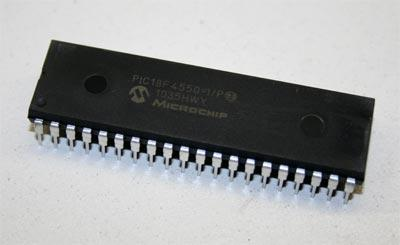
\includegraphics[width=0.4\textwidth]{images/Atividade03/03MicrocontrollerPIC_18F4550.jpg}
\end{figure}

\begin{figure}[ht]
  \centering
  \caption{\label{fig:Atividade-03-05-Schematic-01}Diagrama Esquemático desenvolvido para o PIC18F4550 durante a Atividade~\ref{cha:3-PIC}.}
  \fonte{Produzido pelos autores.}
  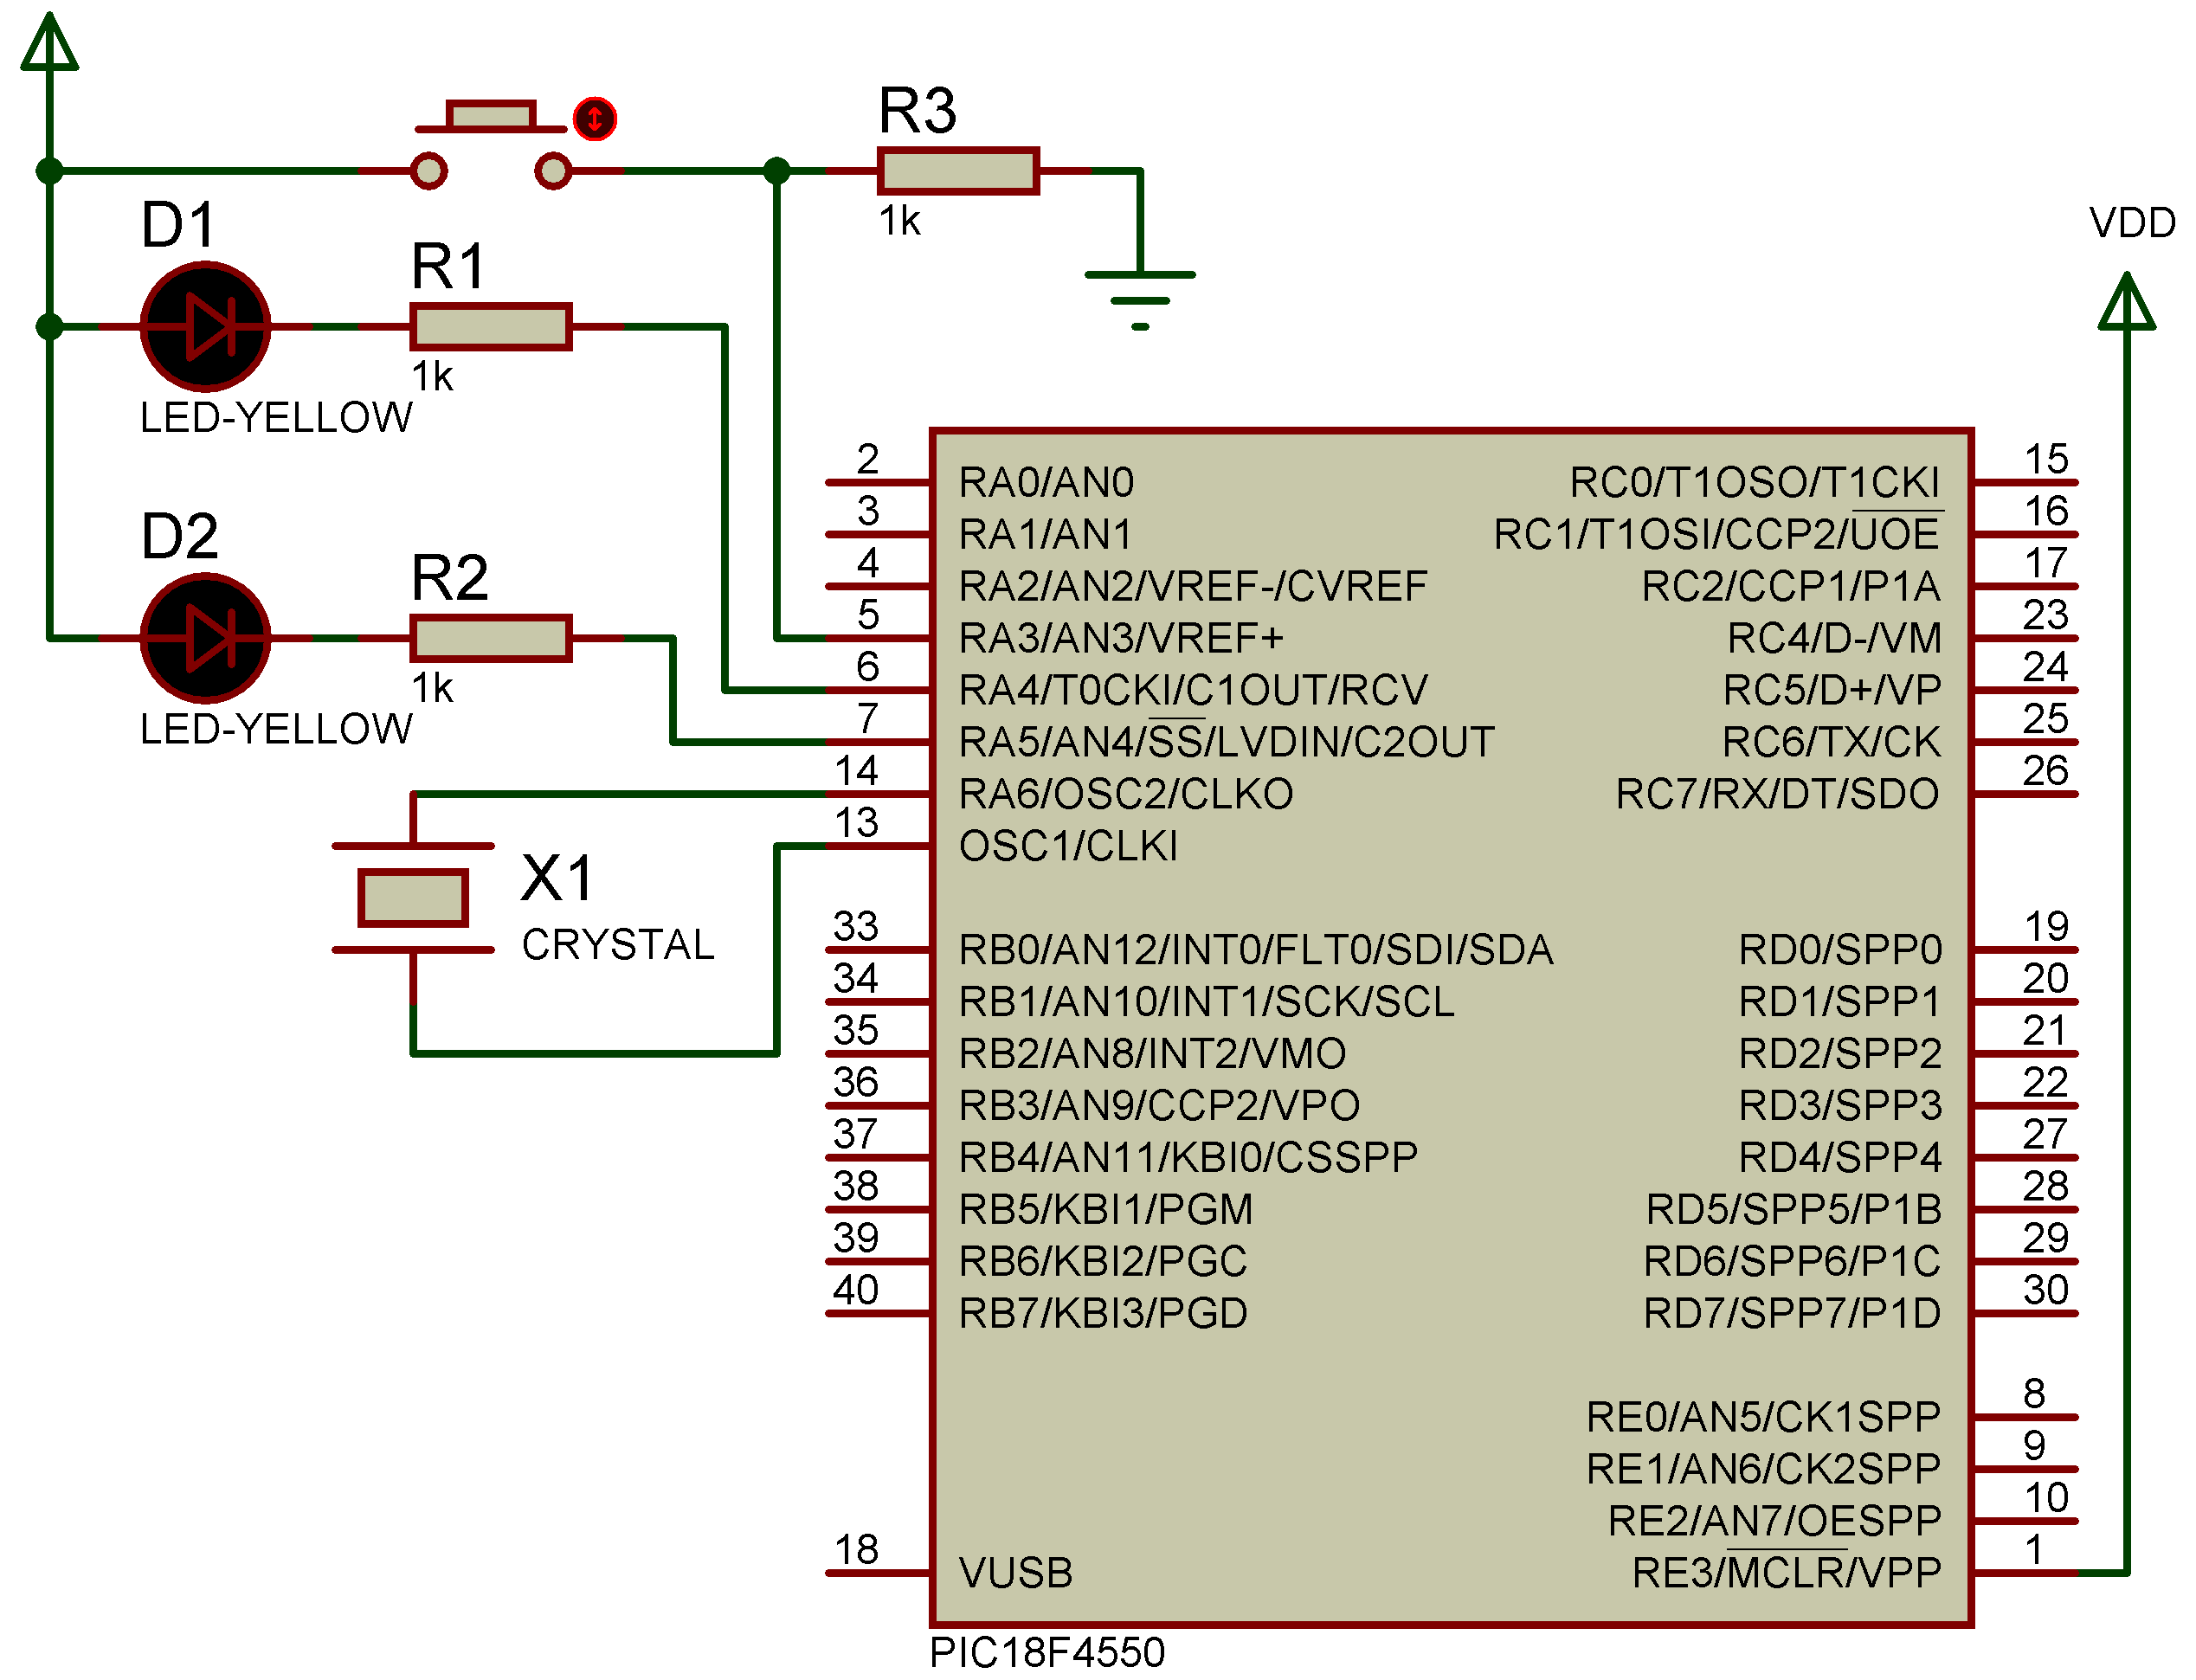
\includegraphics[width=0.9\textwidth]{images/Atividade03/Atividade-03-05-Schematic-01-recortado.png}
\end{figure}

\begin{itemize}
  \item Realizamos a instalação do ProtoN Compiler\footnote{ProtoN Compiler: \url{https://github.com/sftom/ee1054/ide/311-InstallPROTOn.exe}}, e seguimos alguns passos do manual de utilização\footnote{Manual do ProtoN Compiler: \url{https://github.com/sftom/ee1054/ide/311-ManualPROTOn.pdf}};
  \item Em seguida, realizamos a instalação do MikroC Pro PIC 2014\footnote{MikroC Pro PIC 2014\url{https://github.com/sftom/ee1054/ide/312-mikroC_PRO_PIC_2014_Build.6.4.0.exe}} e manual de utilização\footnote{Manual do MikroC Pro PIC 2014\url{https://github.com/sftom/ee1054/ide/312-ManualMikroc-pro-pic.pdf}};
  \item Como pedido na atividade foi utilizado o MicroC e a PROTOn;
\end{itemize}

\begin{figure}[ht]
  \centering
  \caption{\label{fig:cha-3-mikroC-Pro00}Programação em IDE MikroC.}
  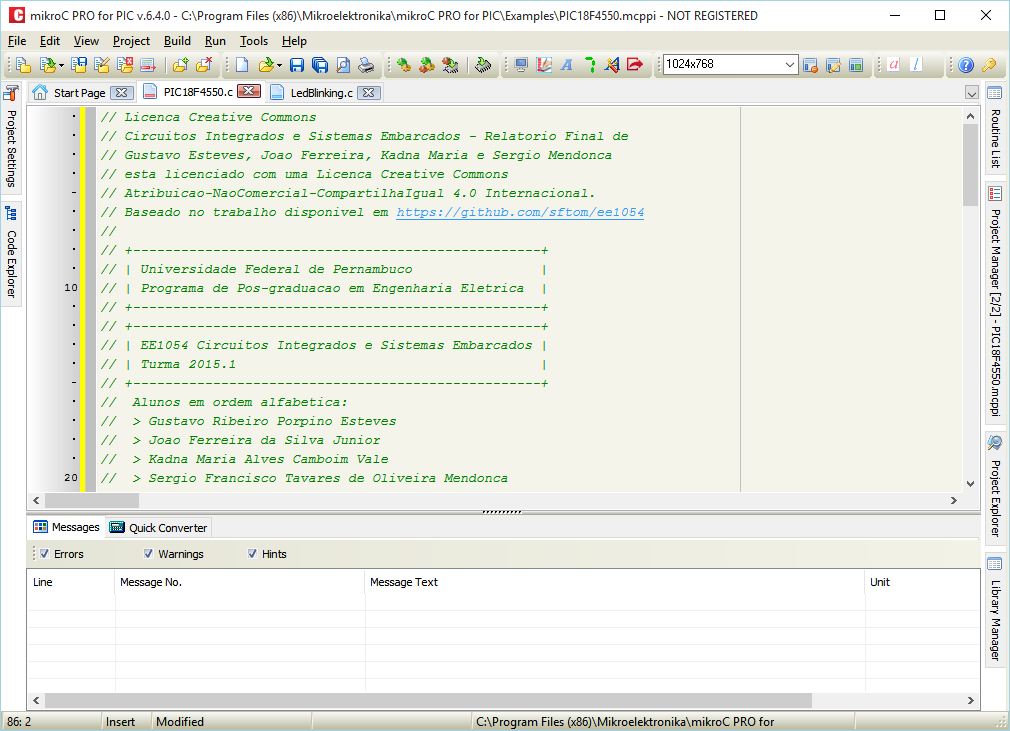
\includegraphics[width=0.8\textwidth]{images/Atividade03/mikroC-PRO00.png}
\end{figure}

\begin{figure}[ht]
  \centering
  \caption{\label{fig:cha-3-mikroC-Pro01}Configuração do microcontrolador na IDE MikroC.}
  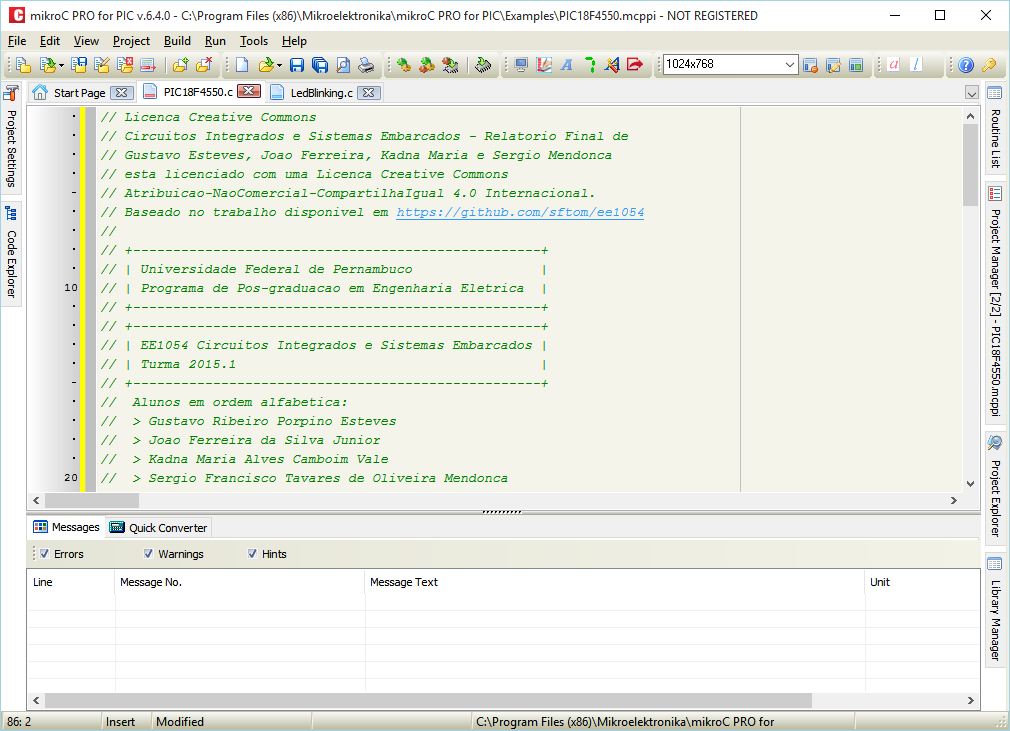
\includegraphics[width=0.8\textwidth]{images/Atividade03/mikroC-PRO00.png}
\end{figure}

\begin{figure}[ht]
  \centering
  \caption{\label{fig:cha-3-PROTOn-BOOTLOADER}Configuração do Bootloader na aplicação \textsc{PROTO'n}.}
  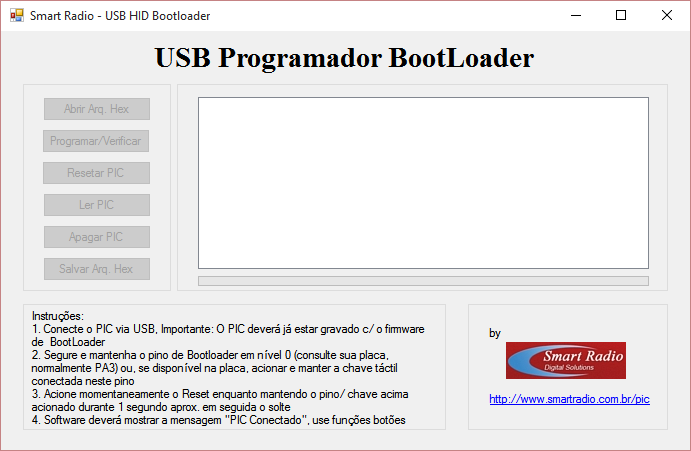
\includegraphics[width=0.8\textwidth]{images/Atividade03/PROTOn-BOOTLOADER.png}
\end{figure}

A gravação dos códigos desenvolvidos no PIC18F4550 é realizada através de um gravador, como mostrado na Figura~\ref{fig:04GravadorPIC}.

\begin{figure}[ht]
  \centering
  \caption{\label{fig:04GravadorPIC}Gravador de firmware para Microcontrolador PIC18F4550.}
  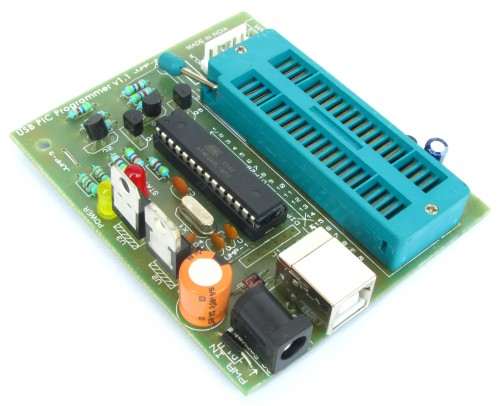
\includegraphics[width=0.6\textwidth]{images/Atividade03/04GravadorPIC.jpg}
\end{figure}

Para fonte de consulta, inserimos o Diagrama de Bloco, como pode ser observado na Figura~\ref{fig:cha-3-diagrama-de-bloco-PIC18F4550}, extraída do Data Sheet do PIC18F4550. \cite{Inc.2009}.

\newpage
%inserindo algumas páginas: 1 até 7, depois 50 e 57

\begin{figure}[H]
  \centering
  \caption{\label{fig:cha-3-diagrama-de-bloco-PIC18F4550}Diagrama de Bloco do Data Sheet do PIC18F4550.}  
  \includepdf[pages=12,frame=true,width=0.95\textwidth,pagecommand={}]{datasheets/A4-A3-02Datasheet-39632e.pdf}
\end{figure}


\newpage

Os códigos-fontes elaborados estão disponibilizados a seguir:

% ----------------------------------------------------------
\section*{Microcontrolador PIC18F4550 -- A03 (Códigos-fontes)}
\label{sec:PIC-A03Q02}
% ----------------------------------------------------------
\subsection*{A03Q02}
\lstinputlisting{sources/EE1054-Atividade03-Questao02-Led.c}

\subsection*{A03Q03}
\lstinputlisting{sources/EE1054-Atividade03-Questao03-Leds-Sequencial.c}




% section considerações_finais (end)

% chapter PIC (end)





%%%%%%%%%%%%%%%%%%%%%%%%%%%%%%%%%%%%%%%%%%%%%%%%%%%%%%%%%%%%%%%%%%%%%%%%%%%%%%%%%%%%%
%
% chapter: Microcontrolador MSP430
%
%%%%%%%%%%%%%%%%%%%%%%%%%%%%%%%%%%%%%%%%%%%%%%%%%%%%%%%%%%%%%%%%%%%%%%%%%%%%%%%%%%%%%%


\chapter{Microcontrolador MSP430}% (fold)
\label{cha:4-MSP430}

\section{Atividades propostas} % (fold)
\label{cha:MSP430-sec:atividades_propostas}

\subsection*{Relatório de experimentos – Aula prática com microcontrolador família MSP430}

\subsubsection*{Atividade 4}

\begin{enumerate}
  \item Instalar o compilador Code Composer Studio (CCS) Integrated Development Environment (IDE\footnote{\url{http://www.ti.com/tool/ccstudio-msp}}) for MSP Microcontrollers.
  \item Realizar testes para piscar LEDs com a placa LAunchPad MSP-exp430G2 e também com a placa eZ430-RF2500T.
  \item Fazer um programa para ler um sinal proveniente de dois botões externos a placa e realizar o acionamento de 4 LEDs, conforme a tabela abaixo (escolher qualquer uma das placas), conforme a Tabela~\ref{Table:MSP430}:
  \begin{table}[h]
    \centering
    \caption{\label{Table:MSP430}Esquema de programação da da MSP430.}
    \begin{tabular}{ccc}
    \hline
    {\textbf{Botão 1}} & {\textbf{Botão 2}} & {\textbf{Acionamento do LED}} \\ \hline
    1             & 0             & LED1                     \\
    0             & 1             & LED2                     \\
    1             & 1             & LED3                     \\
    0             & 0             & LED4                     \\ \hline
    \end{tabular}
  \end{table}

    Os LEDs deverão acender após a combinação realizada e permanecer durante 1 segundo aceso.

  \item Fazer um programa para gerar pulsos em um pino de saída, bem como acender um indicador (LED) ao mesmo tempo. Utilizar duas teclas externas uma para aumentar a velocidade das piscadas do LED e outra para diminuir a velocidade das piscadas do LED. Pede-se o controle de velocidade de 1 a 60 piscadas por minuto.
\end{enumerate}

% section atividades_propostas (end)

\section{Relatório da Atividade} % (fold)
\label{sec:consideracoes}

Para fonte de consulta, inserimos o Diagrama de Bloco, como pode ser observado na Figura~\ref{cha:4-diagrama-bloco-microcontrolador}, extraída do Data Sheet do MSP430. \cite{Instruments2012}.

\begin{figure}[!ht]
  \centering
  \caption{\label{fig:03e04MicrocontroladorEZ430-RF2500T}Microcontrolador EZ430-RF2500T e seu Gravador de Firmware.}  
  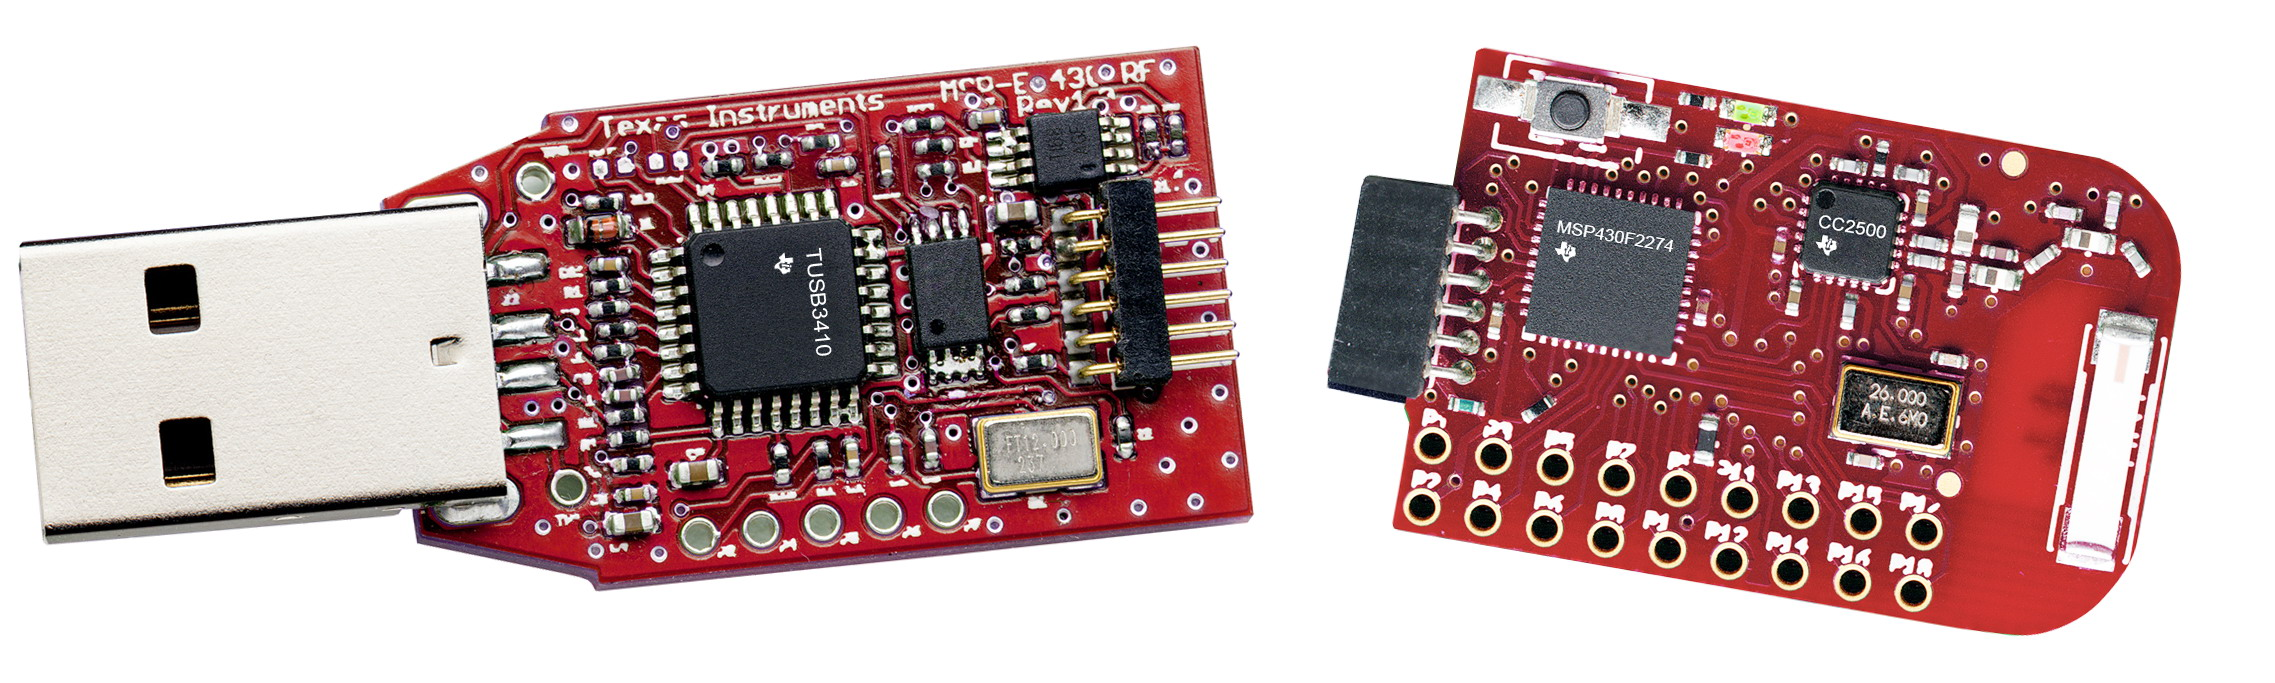
\includegraphics[width=0.6\textwidth]{images/Atividade04/03e04MicrocontroladorEZ430-RF2500T.jpg}
\end{figure}


\begin{figure}[ht]
  \centering
  \caption{\label{fig:Atividade-04-05-Schematic-01-recortado}Diagrama Esquemático desenvolvido para o MSP430F2272 durante a Atividade~\ref{cha:4-MSP430}.}
  \fonte{Produzido pelos autores.}
  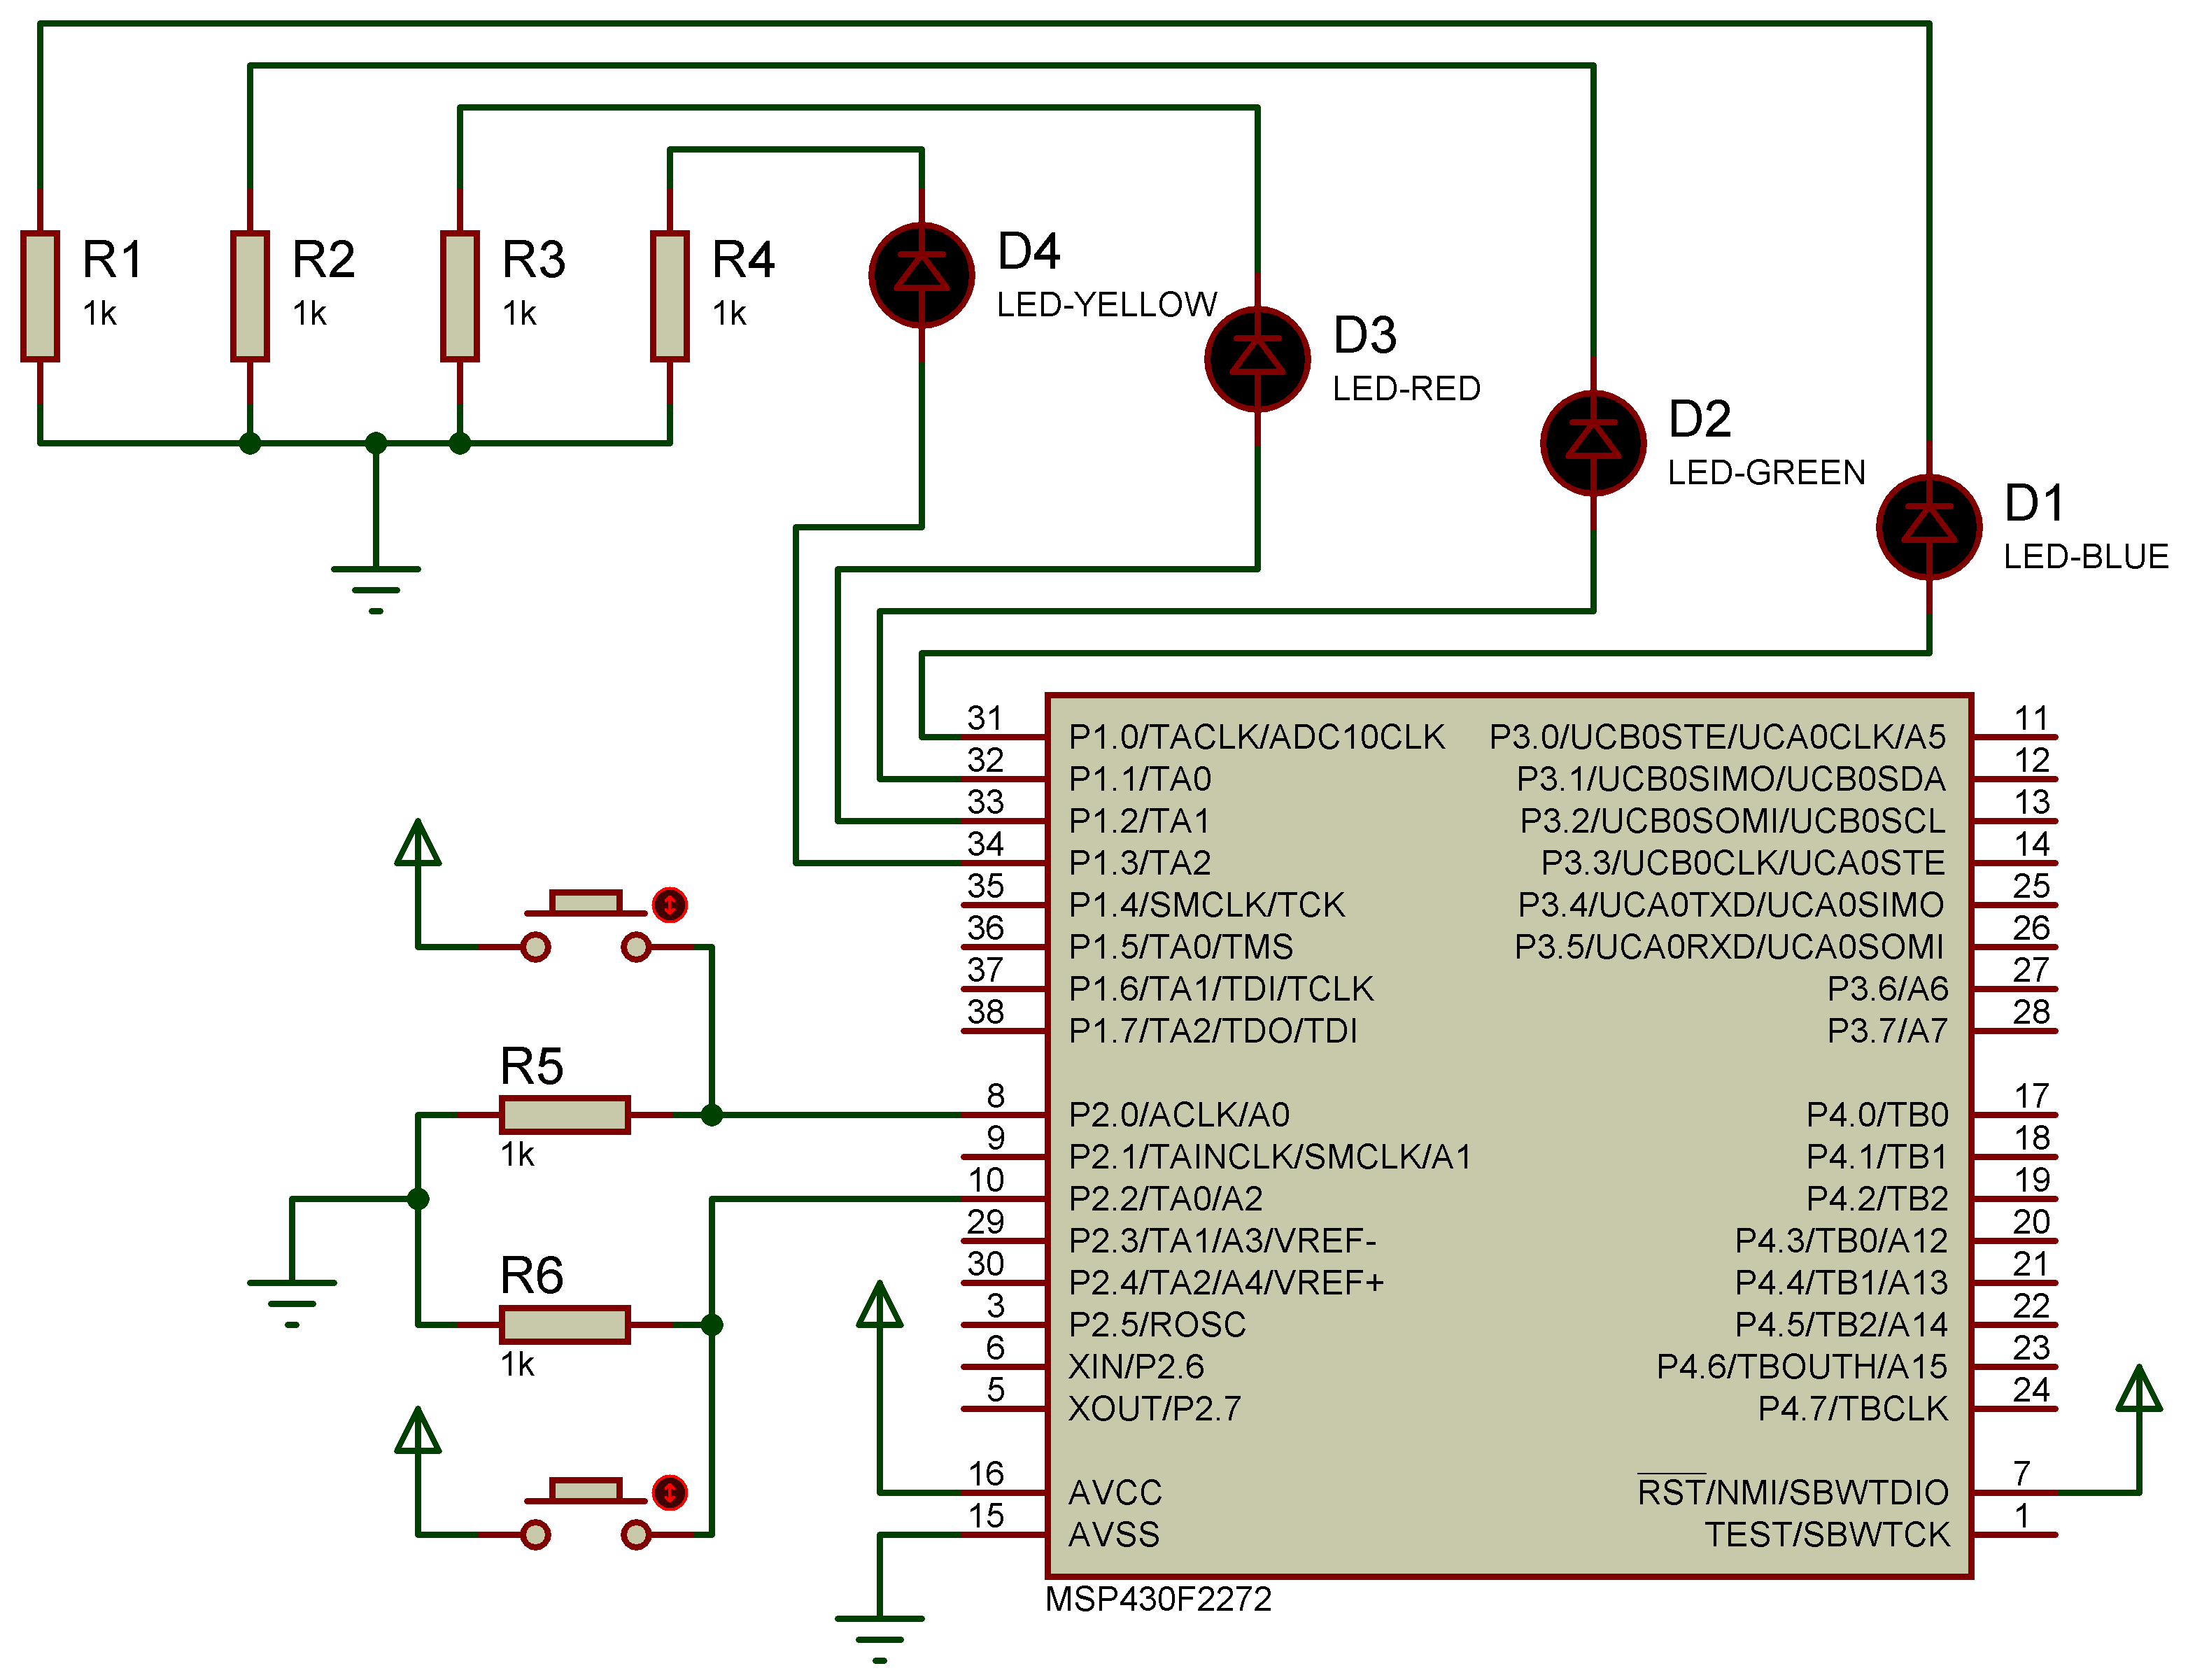
\includegraphics[width=0.8\textwidth]{images/Atividade04/Atividade-04-05-Schematic-01-recortado.png}
\end{figure}

\begin{figure}[ht]
  \centering
  \caption{\label{fig:cha-4-CodeComposer00}Programação do microcontrolador MSP430F2272 na IDE CodeComposer.}
  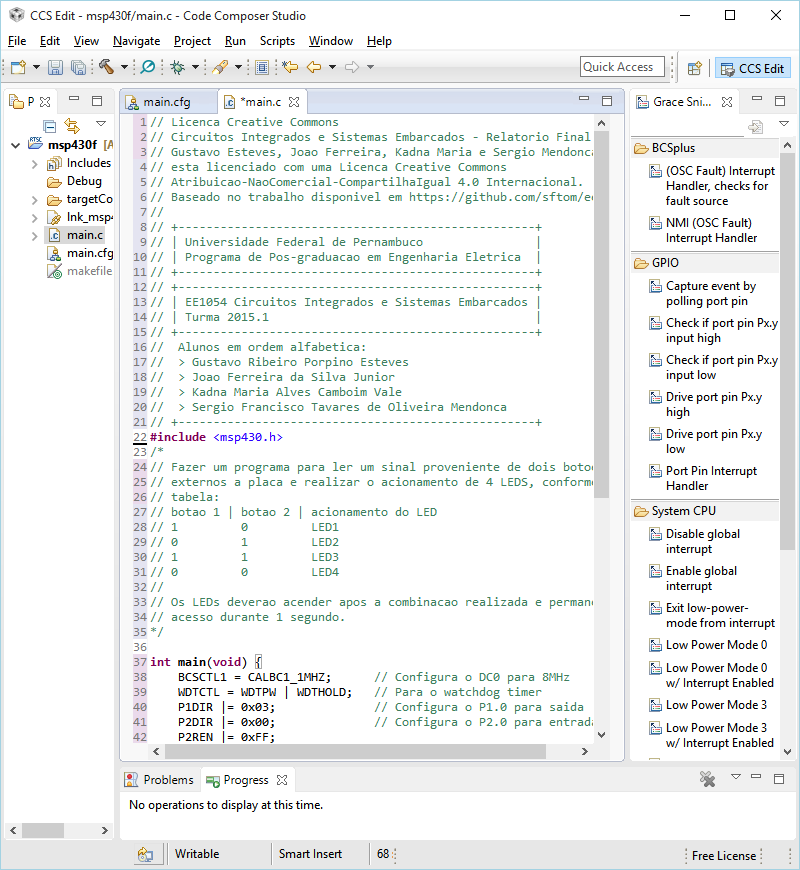
\includegraphics[width=0.8\textwidth]{images/Atividade04/CodeComposer00.png}
\end{figure}

\begin{figure}[ht]
  \centering
  \caption{\label{fig:cha-4-CodeComposer01}Programação do microcontrolador MSP430F2272 na IDE CodeComposer.}
  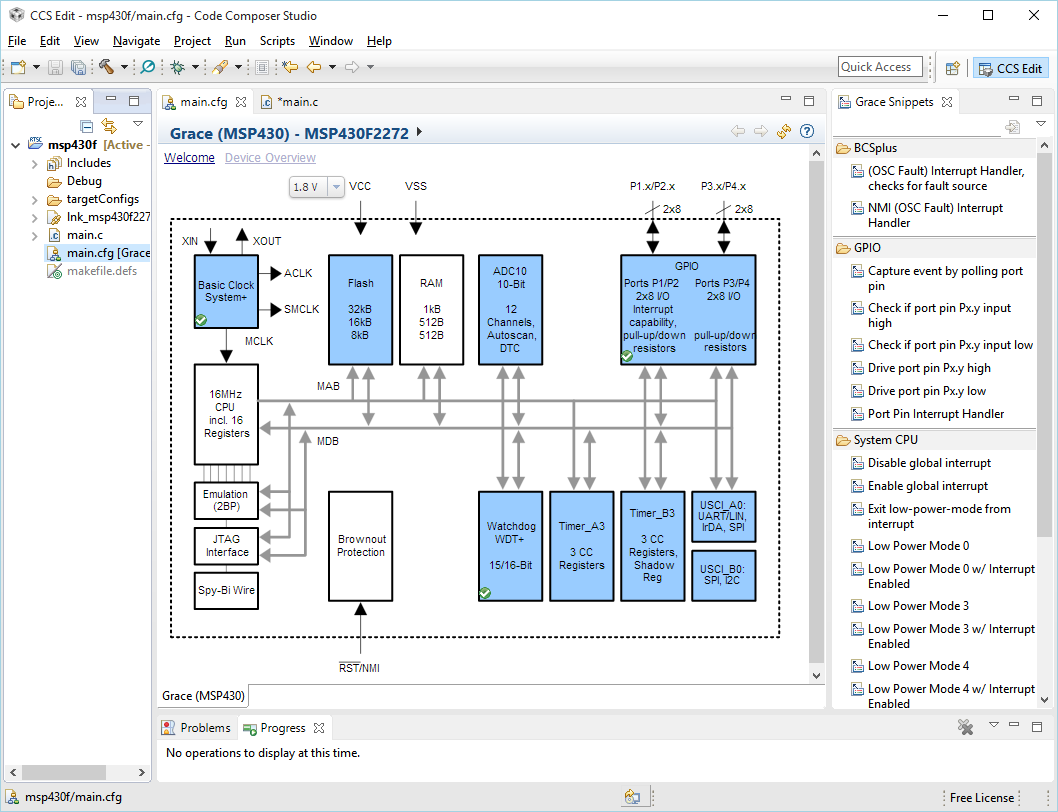
\includegraphics[width=0.8\textwidth]{images/Atividade04/CodeComposer01.png}
\end{figure}

\newpage
%inserindo algumas páginas: 1 até 7, depois 50 e 57
\begin{figure}[H]
  \centering
  \caption{\label{cha:4-diagrama-bloco-microcontrolador}Diagrama de Bloco do Data Sheet do MSP430.}
  \includepdf[pages=7,frame=true,width=0.95\textwidth,pagecommand={}]{datasheets/A4-A4-02Datasheet-msp430f2274.pdf}
\end{figure}

\newpage

Os códigos-fontes elaborados estão disponibilizados a seguir:
% ----------------------------------------------------------
\section*{Microcontrolador MSP430 -- A04 (Códigos-fontes)}
\label{sec:MSP430-A04Q04}
% ----------------------------------------------------------
\subsection*{A04Q04}
\lstinputlisting{sources/EE1054-Atividade04-Questao04-Pulso.c}

% section considerações (end)

% chapter PIC (end)

%%%%%%%%%%%%%%%%%%%%%%%%%%%%%%%%%%%%%%%%%%%%%%%%%%%%%%%%%%%%%%%%%%%%%%%%%%%%%%%%%%%%%
%
% chapter Microcontrolador MSP430 -- GRACE
%
%%%%%%%%%%%%%%%%%%%%%%%%%%%%%%%%%%%%%%%%%%%%%%%%%%%%%%%%%%%%%%%%%%%%%%%%%%%%%%%%%%%%%%

\chapter{Microcontrolador MSP430 -- GRACE} % (fold)
\label{cha:5-msp430_grace}

\section{Atividades propostas} % (fold)
\label{sec:msp430_grace-atividades_propostas}

\subsection*{Relatório de Experimentos -- Aula prática com MSP430 -- GRACE}

\subsubsection*{Atividade 5}

\begin{enumerate}
  \item Instalar a fermenta de desenvolvimento GRACE para a família MSP430 (disponível do site da Texas).
  \item Escolher um microcontrolador da família MSP430 que possua pelo menos um conversor A/D de 10 bits, interface de I/O para periféricos, memória do tipo flash e comunicação serial assíncrona do tipo RS232. Criar um software compatível no CCS, utilizando o GRACE, com as seguintes características:
  \begin{enumerate}
    \item Configurar o conversor A/D para realizar a aquisição de dois canais, com uma taca de 100 amostras por segundo.
    \item Realizar a conversão de 100 amostras, em cada canal.
    \item Gravar as 100 amostras, de cada canal em uma memória FLASH.
    \item Recuperar as 100 amostras, por canal, gravadas na memória FLASH e enviar via comunicação serial, padrão RS232 a uma velocidade de 9600 baunds, para um periférico externo.
  \end{enumerate}
  \item Apresentar um programa completo com as especificações do item 2, com os referidos comentários de como foi realizado todo o processo. Dica: gerar os códigos com o GRACE e posteriormente chamá-los com uma função através do programa principal, construído no CCS.
\end{enumerate}

% section atividades_propostas (end)

\section{Relatório da Atividade} % (fold)
\label{sec:msp430_grace-consideracoes}

Para fonte de consulta, inserimos o Diagrama de Bloco, como pode ser observado na Figura~\ref{fig:cha-5-diagrama-bloco}, extraída do Data Sheet do MSP430F2272 (GRACE). \cite{Instruments2012}.

\begin{figure}[ht]
  \centering
  \caption{\label{fig:Atividade-05-05-Schematic-01}Diagrama Esquemático desenvolvido para o MSP430F2272 (GRACE) durante a Atividade~\ref{cha:5-msp430_grace}.}
  \fonte{Produzido pelos autores.}
  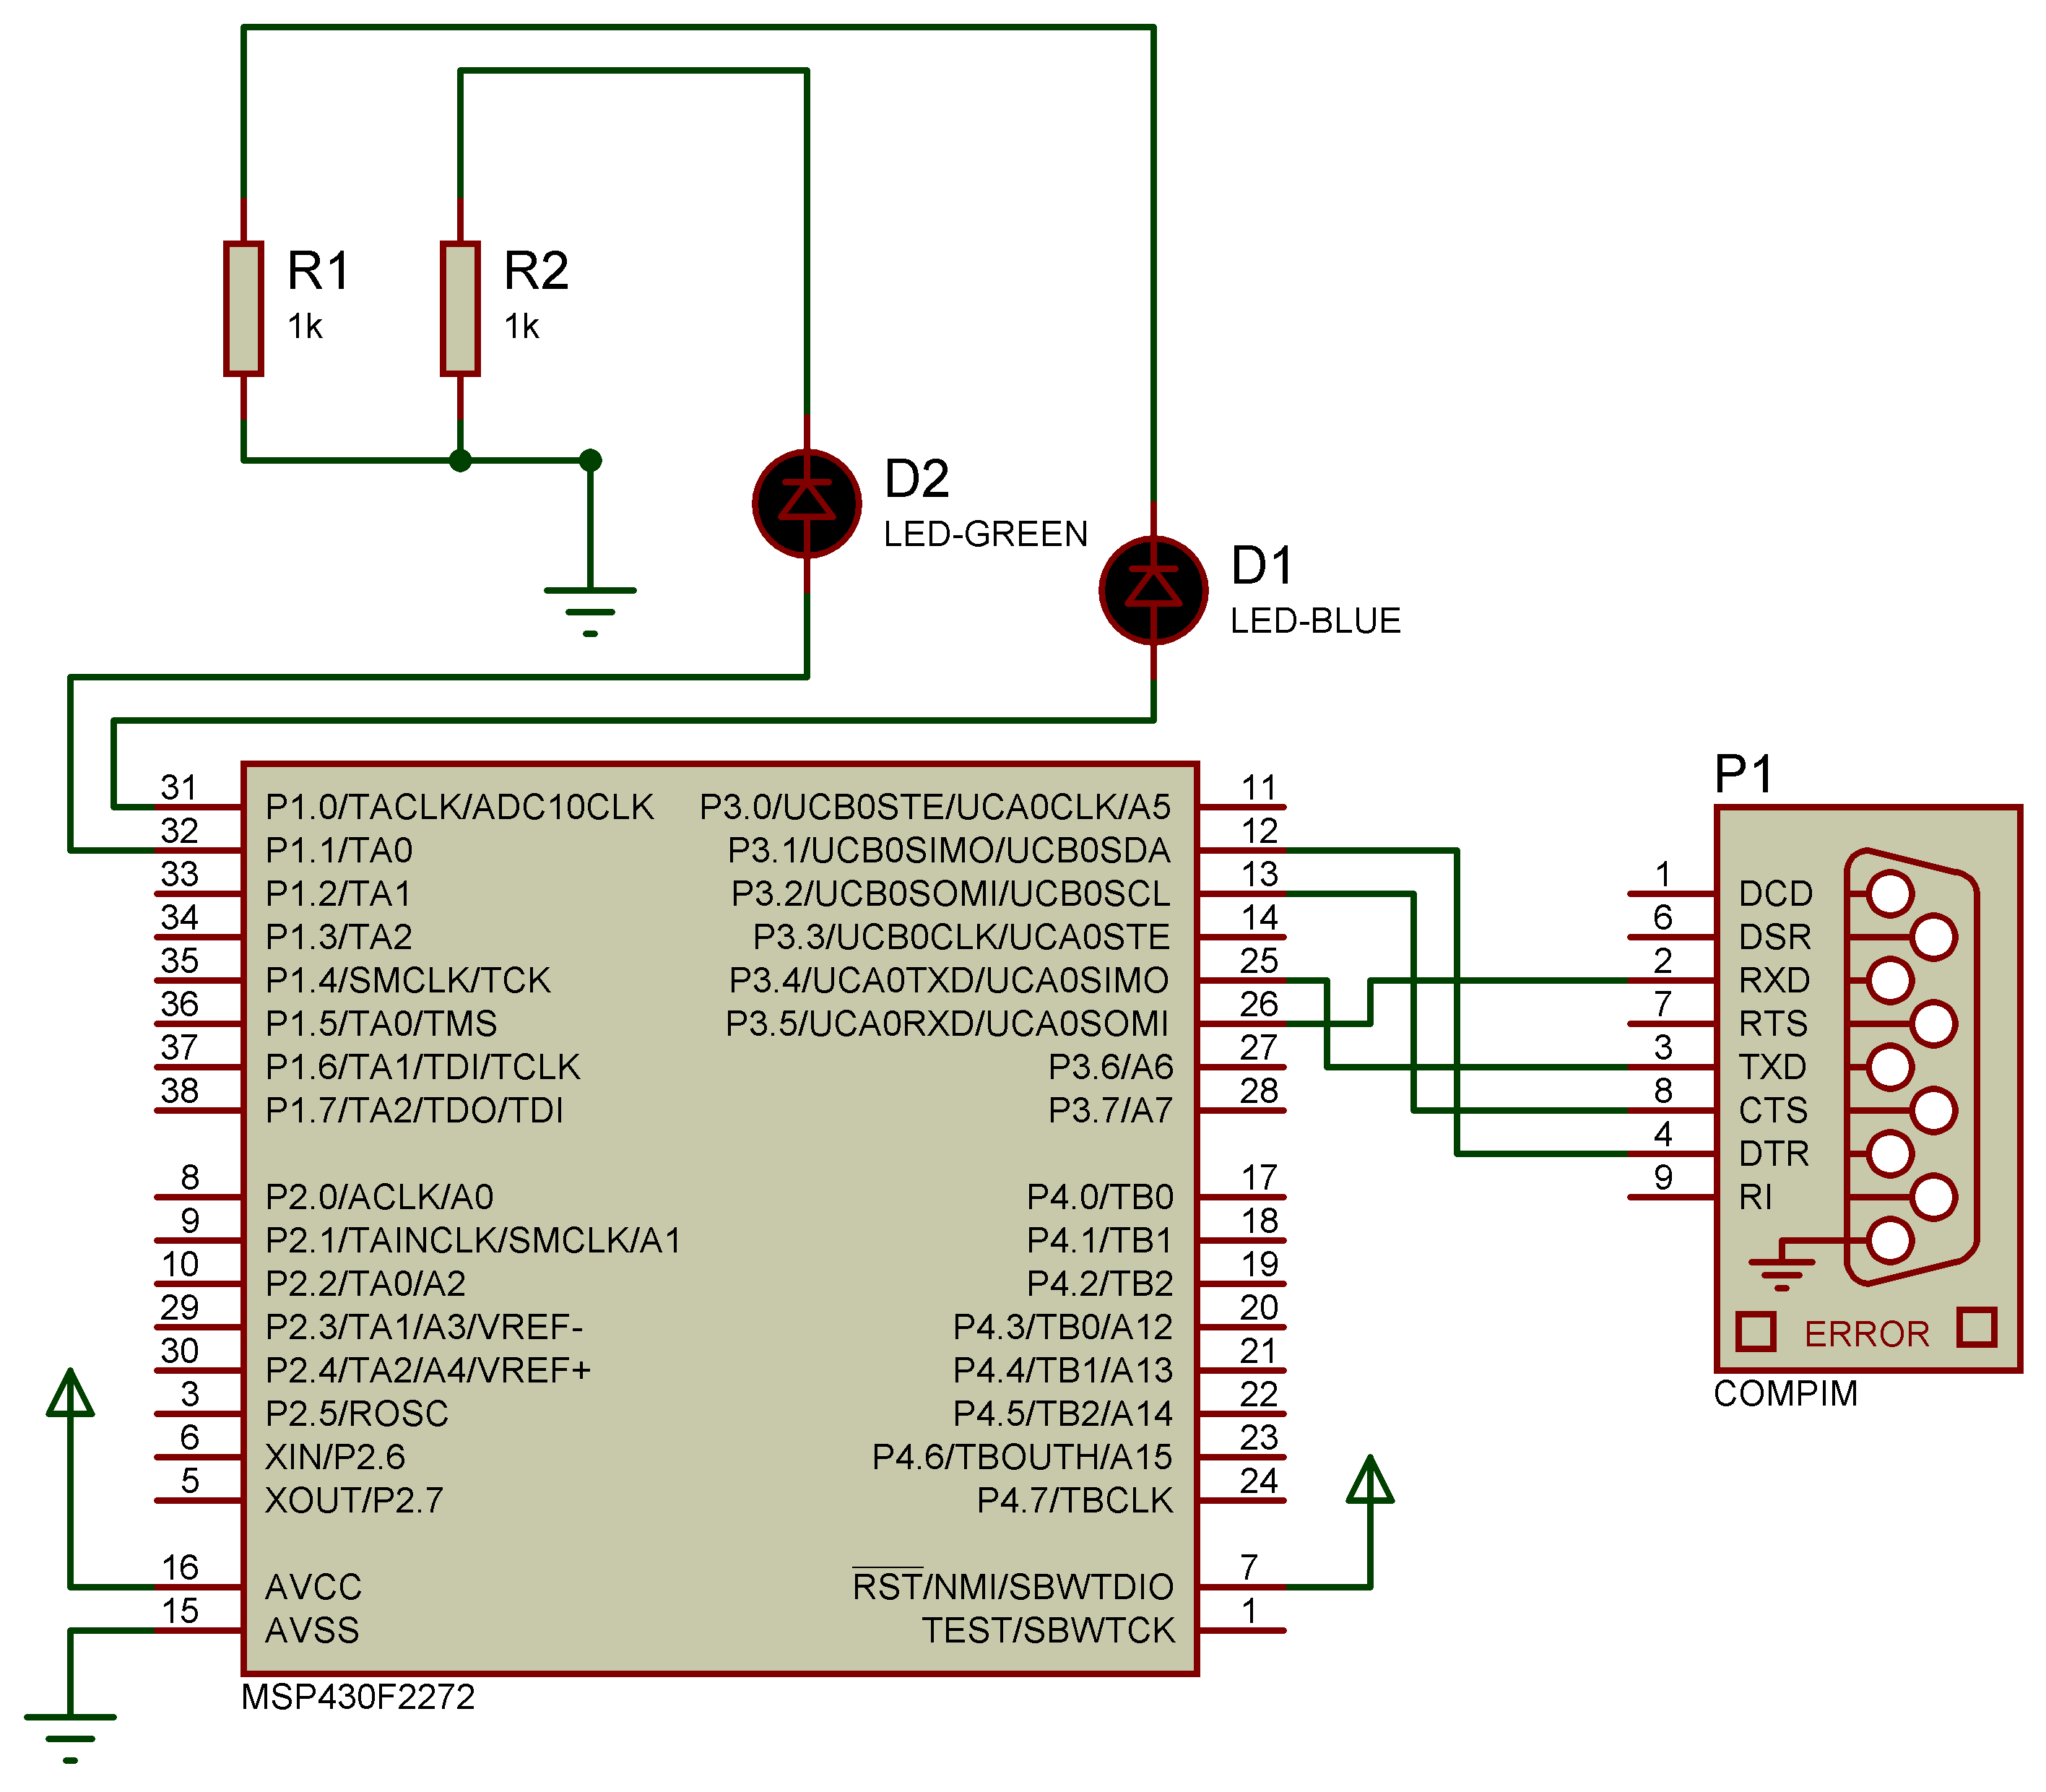
\includegraphics[width=0.8\textwidth]{images/Atividade05/Atividade-05-05-Schematic-01-recortado.png}
\end{figure}

\begin{figure}[ht]
  \centering
  \caption{\label{fig:APP-GRACE00}Programação da MSP430F2272 na IDE GRACE (ambiente de simulação).}
  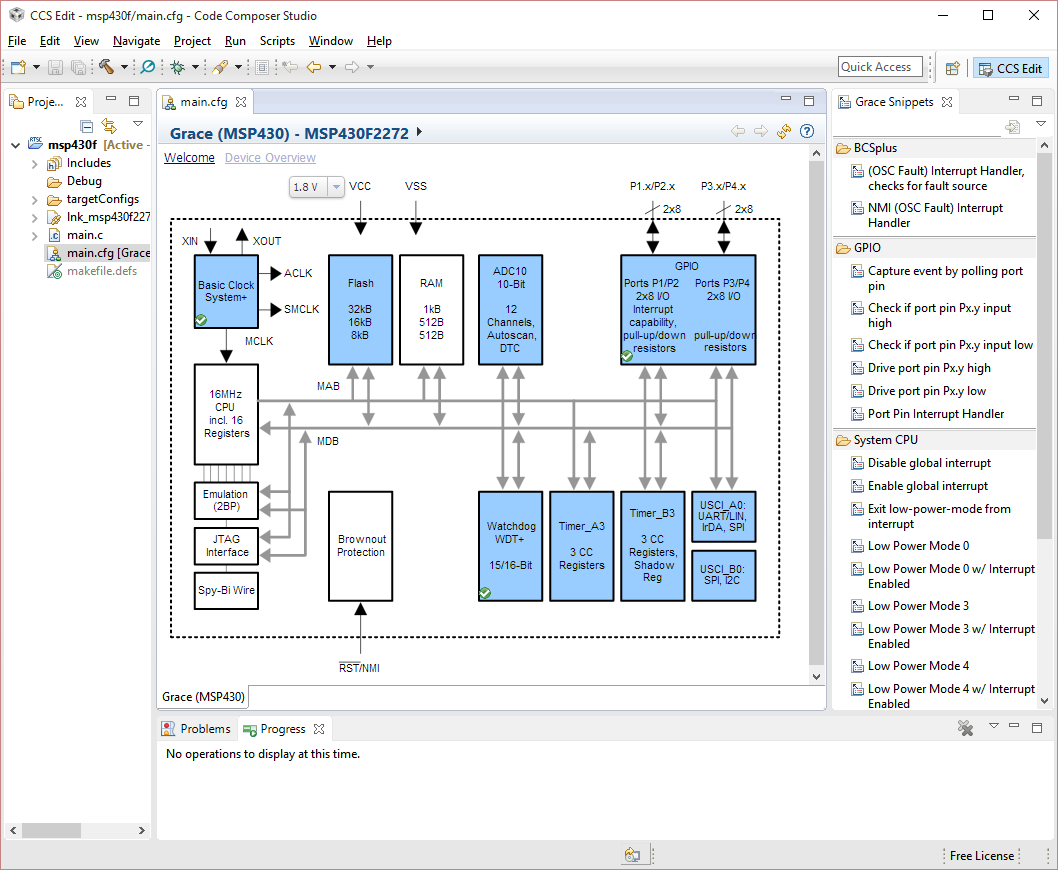
\includegraphics[width=0.8\textwidth]{images/Atividade05/APP-GRACE00.png}
\end{figure}

\begin{figure}[ht]
  \centering
  \caption{\label{fig:APP-GRACE01}Programação da MSP430F2272 na IDE GRACE (ambiente de simulação).}
  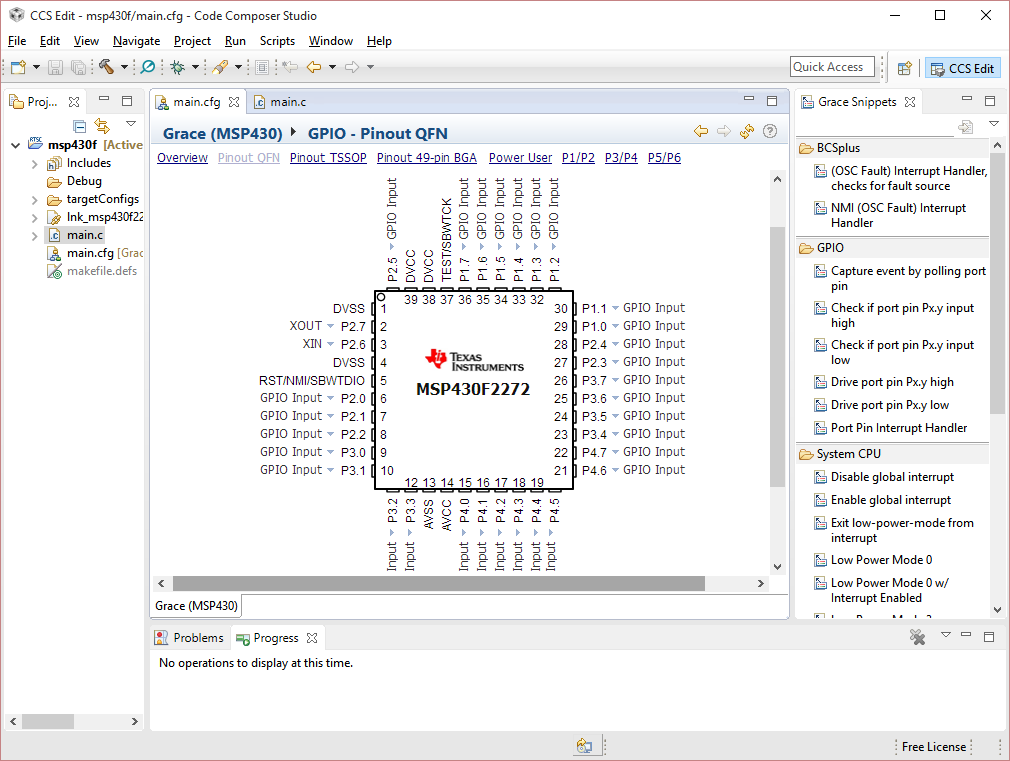
\includegraphics[width=0.8\textwidth]{images/Atividade05/APP-GRACE01.png}
\end{figure}

\begin{figure}[ht]
  \centering
  \caption{\label{fig:APP-GRACE02}Programação da MSP430F2272 na IDE GRACE (ambiente de simulação).}
  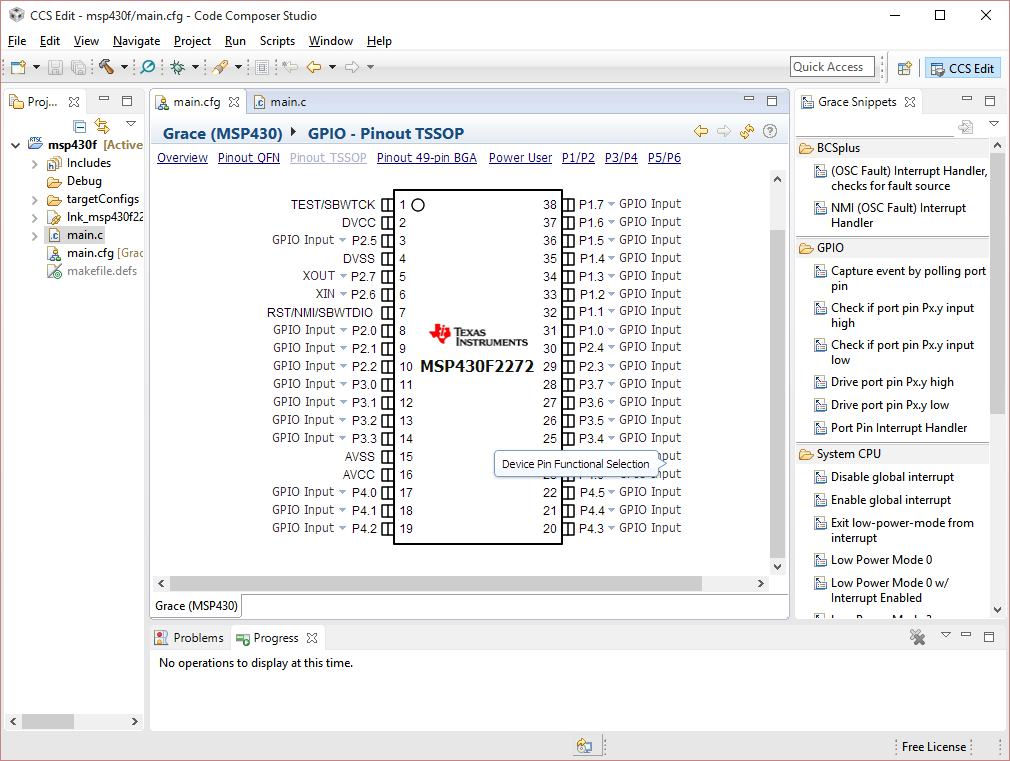
\includegraphics[width=0.8\textwidth]{images/Atividade05/APP-GRACE02.png}
\end{figure}

\newpage
%inserindo algumas páginas: 1 até 7, depois 50 e 57
\begin{figure}[H]
  \centering
  \includepdf[pages=7,width=0.95\textwidth,frame=true,pagecommand={}]{datasheets/A4-A4-02Datasheet-msp430f2274.pdf}
  \caption{\label{fig:cha-5-diagrama-bloco}Diagrama de Bloco do Data Sheet do MSP430.}  
\end{figure}

\newpage
Os códigos-fontes elaborados estão disponibilizados a seguir:
% ----------------------------------------------------------
\section*{MSP430 -- Grace -- A05 (Códigos-fontes)}
\label{sec:GraceA05Q03}
% ----------------------------------------------------------
\subsection*{A05Q02-03}

\lstinputlisting{sources/EE1054-Atividade05-adc_flash_serial.c}

\lstinputlisting{sources/EE1054-Atividade05-BCSplus_init.c}

\lstinputlisting{sources/EE1054-Atividade05-USCI_A0_init.c}



% section considerações_finais (end)

% chapter microcontrolador_msp430_grace (end)


%%%%%%%%%%%%%%%%%%%%%%%%%%%%%%%%%%%%%%%%%%%%%%%%%%%%%%%%%%%%%%%%%%%%%%%%%%%%%%%%%%%%%
%
% chapter: Microcontrolador Kinetis Freescale
%
%%%%%%%%%%%%%%%%%%%%%%%%%%%%%%%%%%%%%%%%%%%%%%%%%%%%%%%%%%%%%%%%%%%%%%%%%%%%%%%%%%%%%%

\chapter{Microcontrolador Kinetis Freescale FRDM-KL25Z} % (fold)
\label{cha:6-microcontrolador_kinetis_freescale}

\section{Atividades propostas} % (fold)
\label{sec:kinetis_freescale-atividades_propostas}

\subsection*{Relatório de Experimentos -- Microcontrolador família Kinetis Freescale}

\subsubsection*{Atividade 6}

\begin{enumerate}
  \item Desenvolver um programa para realizar as seguintes funções com a placa FRDM KL25 fornecida:
  \begin{enumerate}
    \item Ao pressionar uma tecla acender o LED, ao pressionar a segunda vez o LED desliga.
    \item Utilizar um timer para acender um LED, esperar um segundo com ele aceso e depois trocar para a segunda cor do LED, esperar mais um segundo e trocar novamente a cor, para a terceira cor do LED. Reiniciar o processo.
    \item Utilizando o teclado touch da placa, fazer acender o LED e trocar de cores conforme o deslocamento pelo touch.
  \end{enumerate}
\end{enumerate}

% section atividades_propostas (end)

\section{Relatório da Atividade} % (fold)
\label{sec:kinetis_freescale-consideracoes}

Nessa atividade foi escolhido elaborar os códigos a partir do compilador Mbed. Para isso é preciso gravar o bootload adequado na FRDM KL25, ou seja, colocar a FRDM KL25 em modo de gravação de bootload segurando o botão entre seus conectores, plugar a placa a um PC através do conector SDA e passar o arquivo. Após isso os códigos podem ser elaborados diretamente no site da Mbed que possui um compilador web que gera os arquivos a serem gravados na FRDM KL25 através da conexão USB como se estivesse passando arquivos para um Pendrive.

O passo a passo da gravação do bootload da Mbed pode ser encontrado em seu site próprio\footnote{\url{https://developer.mbed.org/handbook/mbed-FRDM-KL25Z-Getting-Started}}.

Para fonte de consulta, inserimos o Diagrama de Bloco, como pode ser observado na Figura~\ref{fig:cha-6-diagrama-bloco-freescale}, extraída do Data Sheet do Kinetis Freescale. \cite{FreescaleSemiconductor2013}.

\begin{figure}[ht]
  \centering
  \caption{\label{fig:kinetis_freescale}Plataforma de desenvolvimento Kinetis Freescale utilizada na Atividade 6.}
  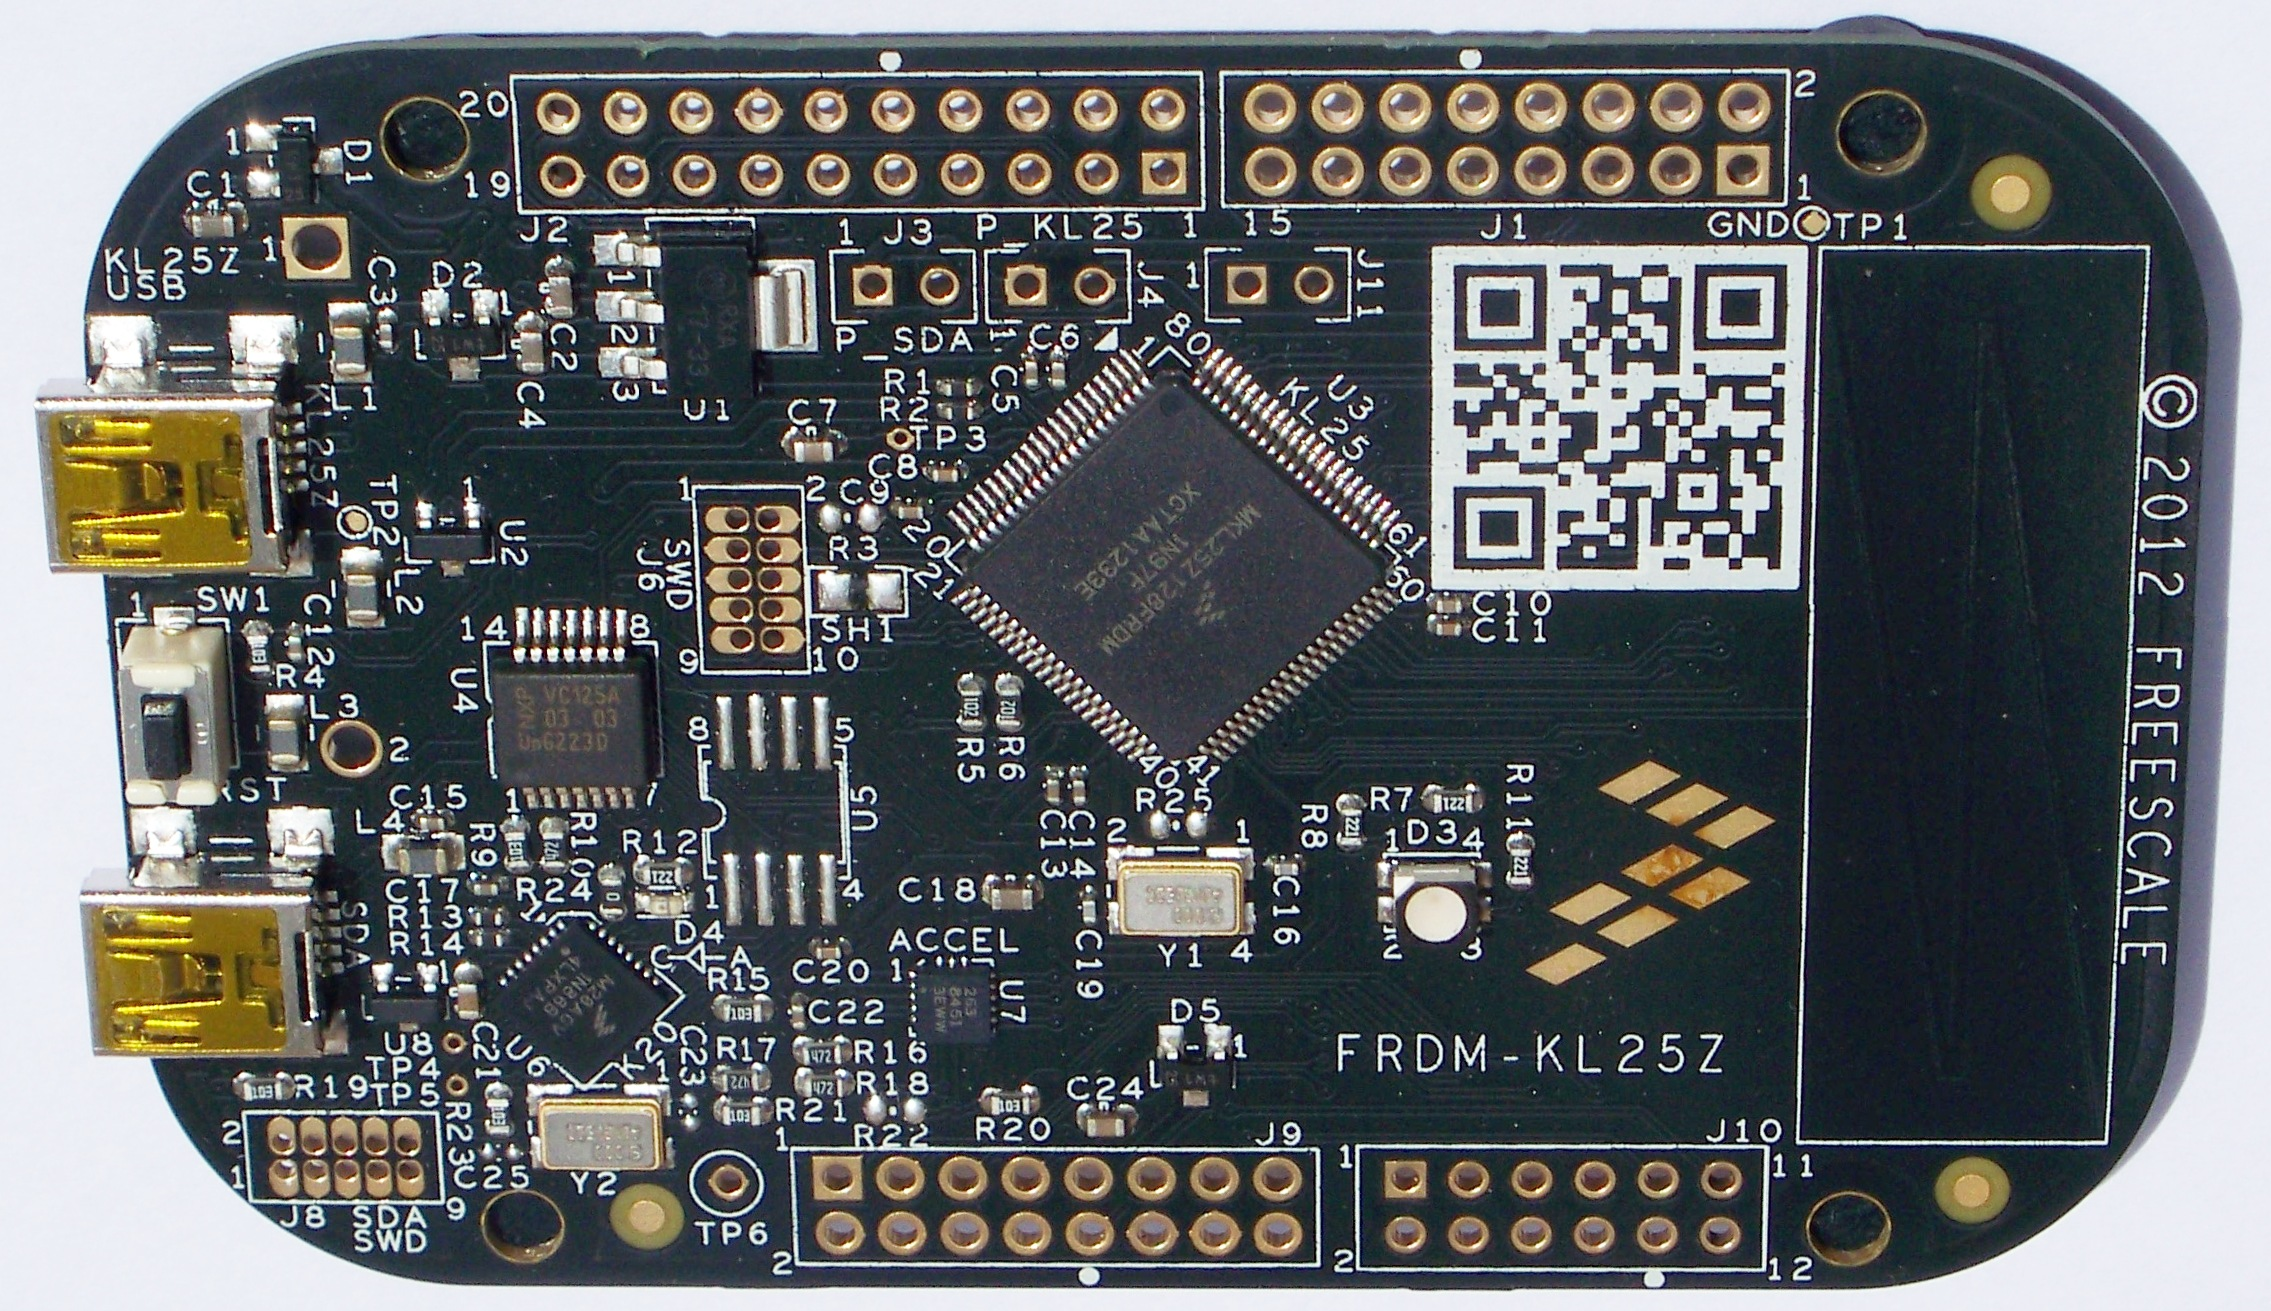
\includegraphics[width=0.7\textwidth]{images/Atividade06/Freescale_FRDM-KL25Z_board_with_KL25Z128VLK_(ARM_Cortex-M0+_MCU).jpg}
\end{figure}

\begin{figure}[ht]
  \centering
  \caption{\label{fig:cha:6-05Schematic_bb}Diagrama Esquemático desenvolvido para o Kinetis Freescale durante a Atividade~\ref{cha:6-microcontrolador_kinetis_freescale}.}
  \fonte{Produzido pelos autores.}
  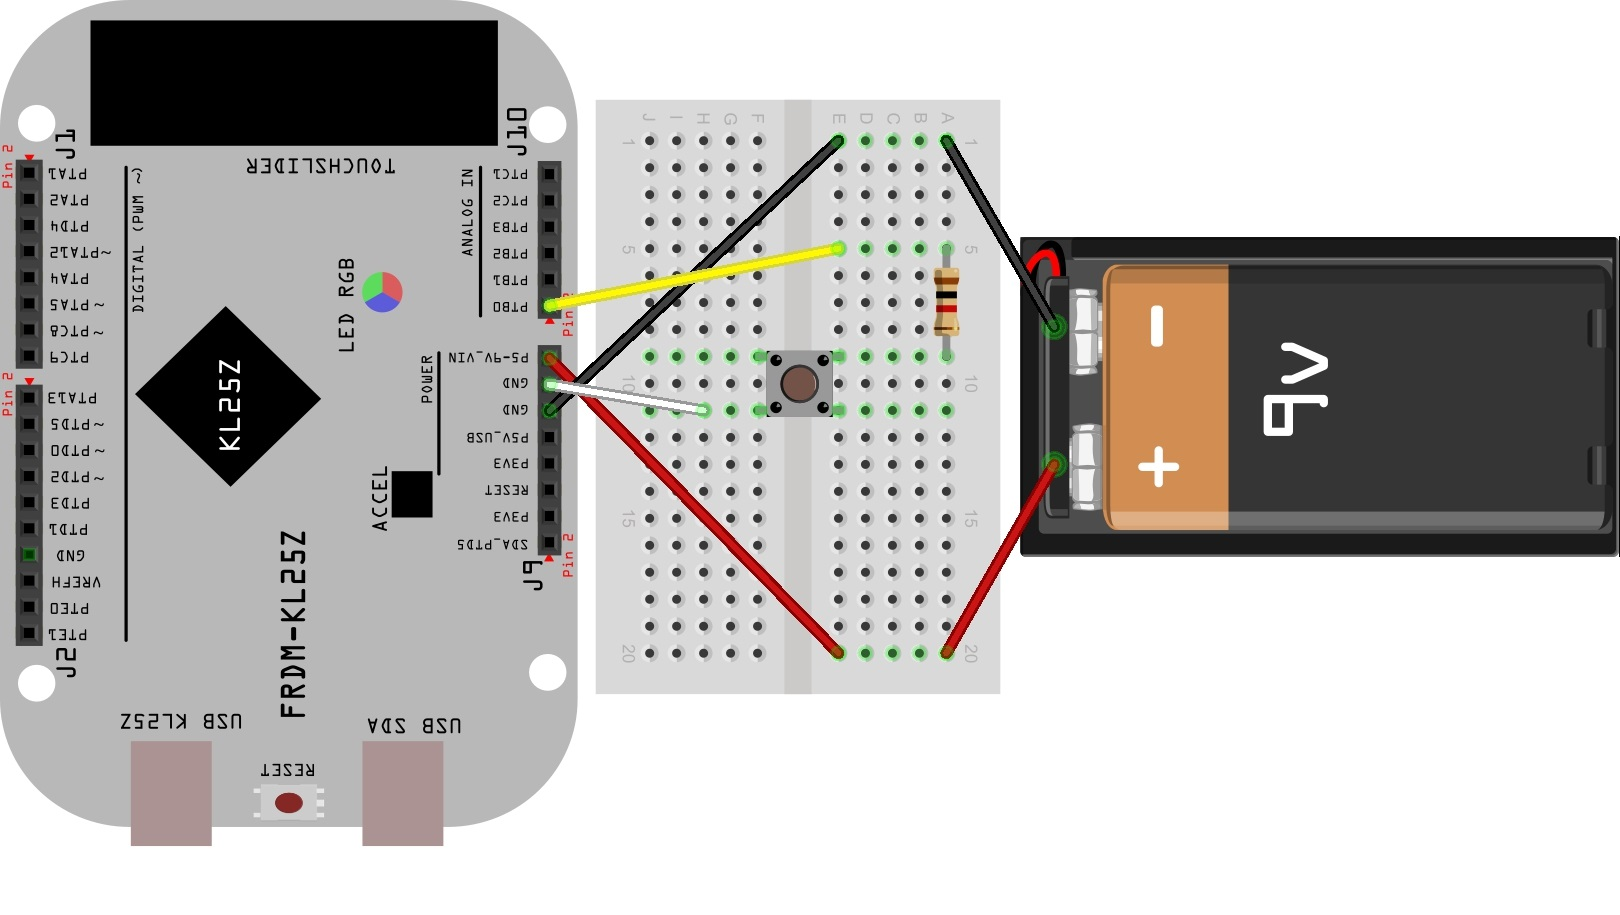
\includegraphics[width=0.8\textwidth]{images/Atividade06/05Schematic_bb.jpg}
\end{figure}

\newpage
%inserindo algumas páginas: 1 até 7, depois 50 e 57
\begin{figure}[H]
  \centering
  \includepdf[pages=4,width=0.95\textwidth,frame=true,pagecommand={}]{datasheets/A4-A6-02Datasheet-FRDM-KL25ZUserManual-Rev-2.pdf}
  \caption{\label{fig:cha-6-diagrama-bloco-freescale}Diagrama de Bloco do Data Sheet do Kinetis Freescale.}
\end{figure}

\begin{figure}[ht]
  \centering
  \caption{\label{fig:cha:APP_KINETS.png}Programação da placa Kinetis Freescale FRDM-KL25Z.}
  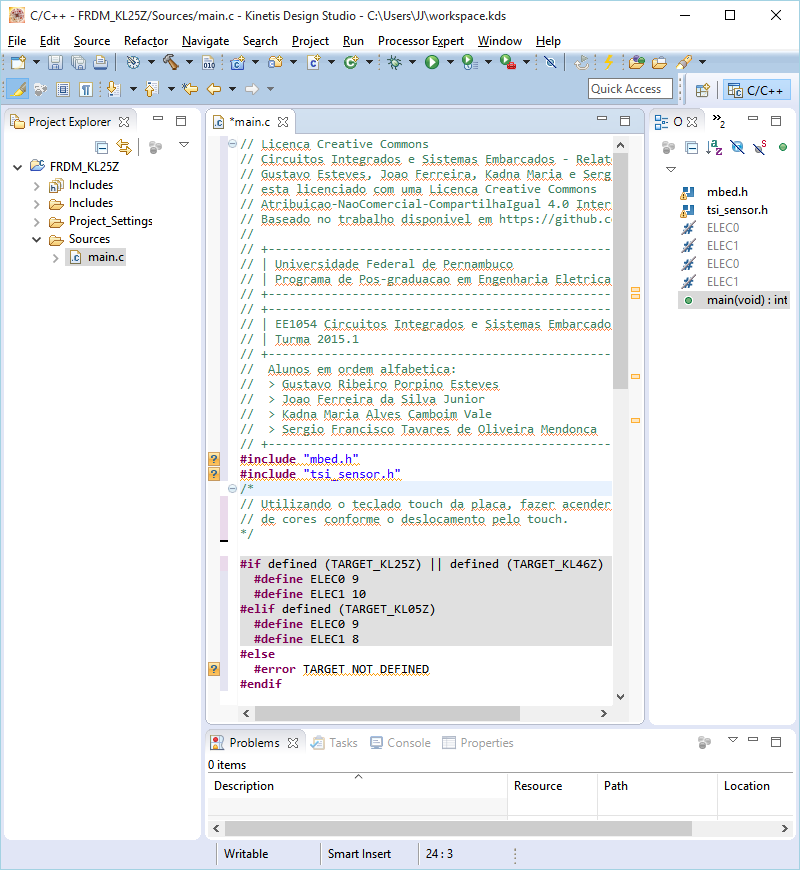
\includegraphics[width=0.8\textwidth]{images/Atividade06/APP_KINETS.png}
\end{figure}

\newpage
Os códigos-fontes elaborados estão disponibilizados a seguir:
% ----------------------------------------------------------
\section*{Microcontrolador Kinetis Freescale -- A06 (Códigos-fontes)}
\label{sec:Kinetis-Freescale-A06Q01-a}
% ----------------------------------------------------------
\subsection*{A06Q01-a}
\lstinputlisting{sources/EE1054-Atividade06-Questao01a-Led.cpp}

\subsection*{A06Q01-b}
\lstinputlisting{sources/EE1054-Atividade06-Questao01b-Timer.cpp}

\subsection*{A06Q01-c}
\lstinputlisting{sources/EE1054-Atividade06-Questao01c-Touch.cpp}

% section considerações_finais (end)

% chapter microcontrolador_kinetis_freescale (end)

%%%%%%%%%%%%%%%%%%%%%%%%%%%%%%%%%%%%%%%%%%%%%%%%%%%%%%%%%%%%%%%%%%%%%%%%%%%%%%%%%%%%%
%
% chapter: Placa Raspberry Pi B+
%
%%%%%%%%%%%%%%%%%%%%%%%%%%%%%%%%%%%%%%%%%%%%%%%%%%%%%%%%%%%%%%%%%%%%%%%%%%%%%%%%%%%%%%

\chapter{Placa Raspberry Pi B+} % (fold)
\label{cha:7-placa_raspberry_pi}

\section{Atividades propostas} % (fold)
\label{sec:RaspberryPi-atividades_propostas}

\subsection*{Trabalho final da disciplina}

\subsubsection*{Atividade 7}

\begin{enumerate}
  \item Utilizando a placa Raspberry Pi, instalar o sistema operacional, linguagem Python 3 e editor de código.
  \item Fazer um programa em Python para apresentar na tela a informação da disciplina e dos integrantes do grupo.
  \item Fazer um programa para ler a temperatura e umidade, através do sensor fornecido. Apresentar os resultados em tela.
  \item Fazer um programa para configurar o display de cristal líquido fornecido. Apresentar a mesma informação de temperatura e umidade na tela do display.
  \item Apresentar um relatório completo sobre todos os itens solicitados com o esquemático de ligação dos componentes.
\end{enumerate}

\noindent OBS: Para finalização da disciplina pede-se:

\begin{enumerate}
  \item Relatório de todos os trabalhos desenvolvidos, informando a tecnologia utilizada, compilador, etc (PDF e DOC).
  \item Anexo com todos os códigos desenvolvidos nos trabalhos (todos os códigos fontes).
  \item Gravação do material em um DVD, identificando os componentes do grupo.
\end{enumerate}


% section atividades_propostas (end)

\section{Relatório da Atividade} % (fold)
\label{sec:consideracoes-RaspberryPi}

Primeiramente o sistema operacional Raspibian foi gravado em um cartão SD seguindo os passos que podem ser encontrados no Manual\footnote{\url{https://www.raspberrypi.org/help/noobs-setup}}. 

Para fonte de consulta, inserimos o Diagrama Pinout da Placa Raspberry Pi B+, como pode ser observado na Figura~\ref{fig:cha-7-diagrama-pinout}, extraída do Manual do Usuário. \cite{System2015}.

\begin{figure}[!ht]
  \centering
  \caption{\label{fig:RaspberryBPlus}Raspberry B+ utilizada na Atividade 7.}
  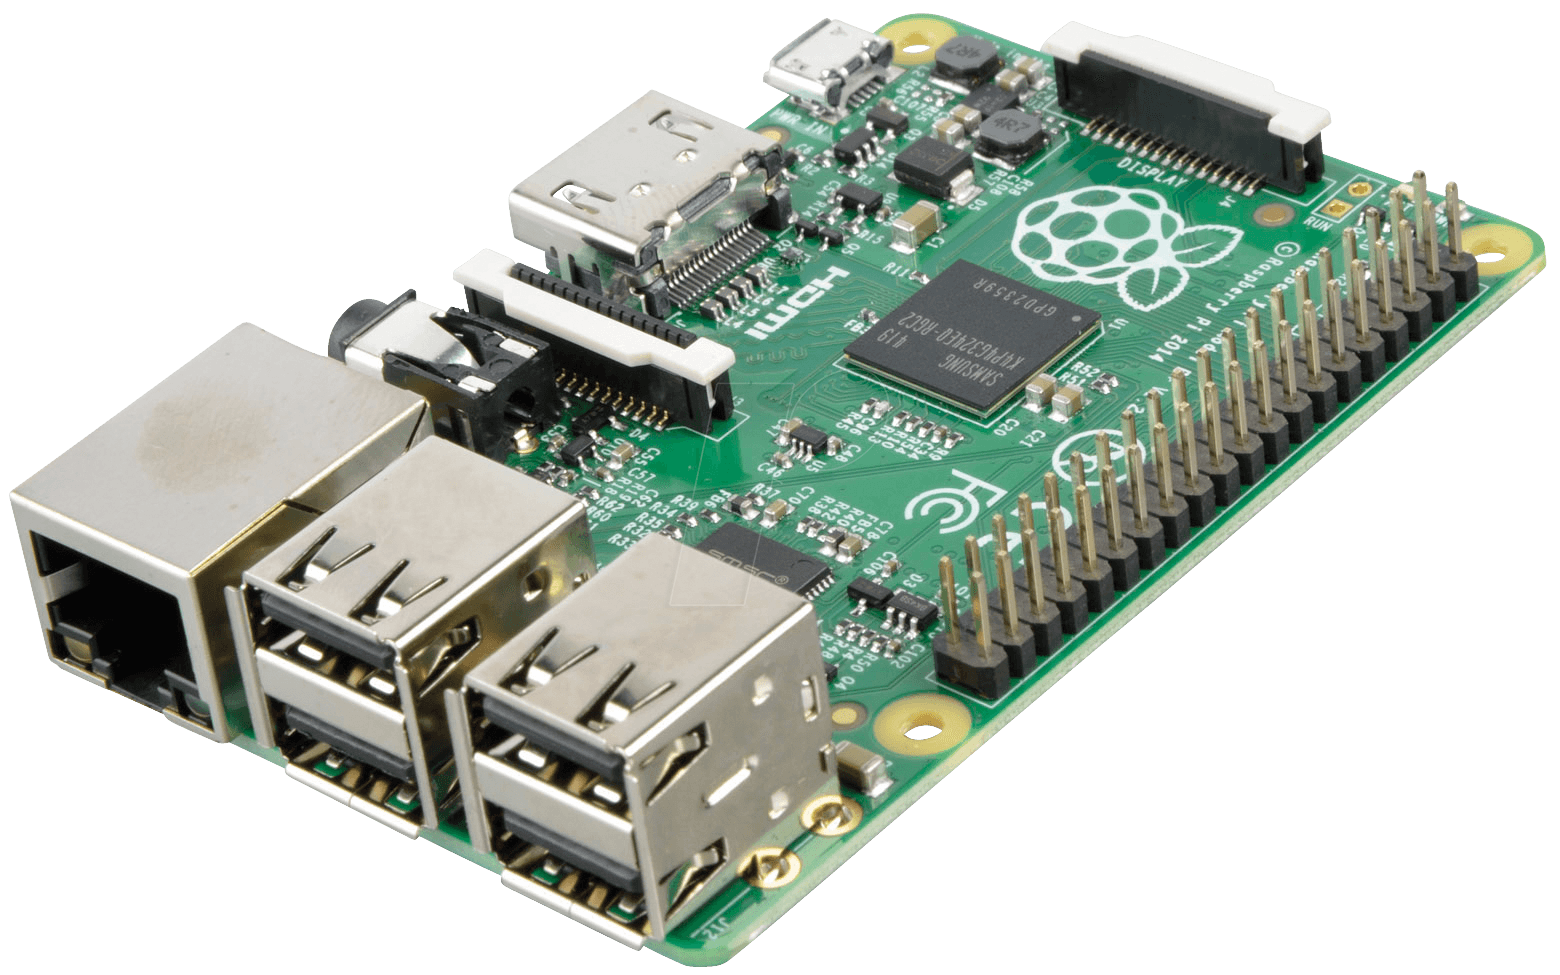
\includegraphics[width=0.5\textwidth]{images/Atividade07/RASPBERRY_PI_B_PLUS_02(1).png}
\end{figure}

\begin{figure}[!ht]
  \centering
  \caption{\label{fig:03e04DisplayLCD}Modelo de LCD utilizado na prática com Raspberry Pi B+.}
  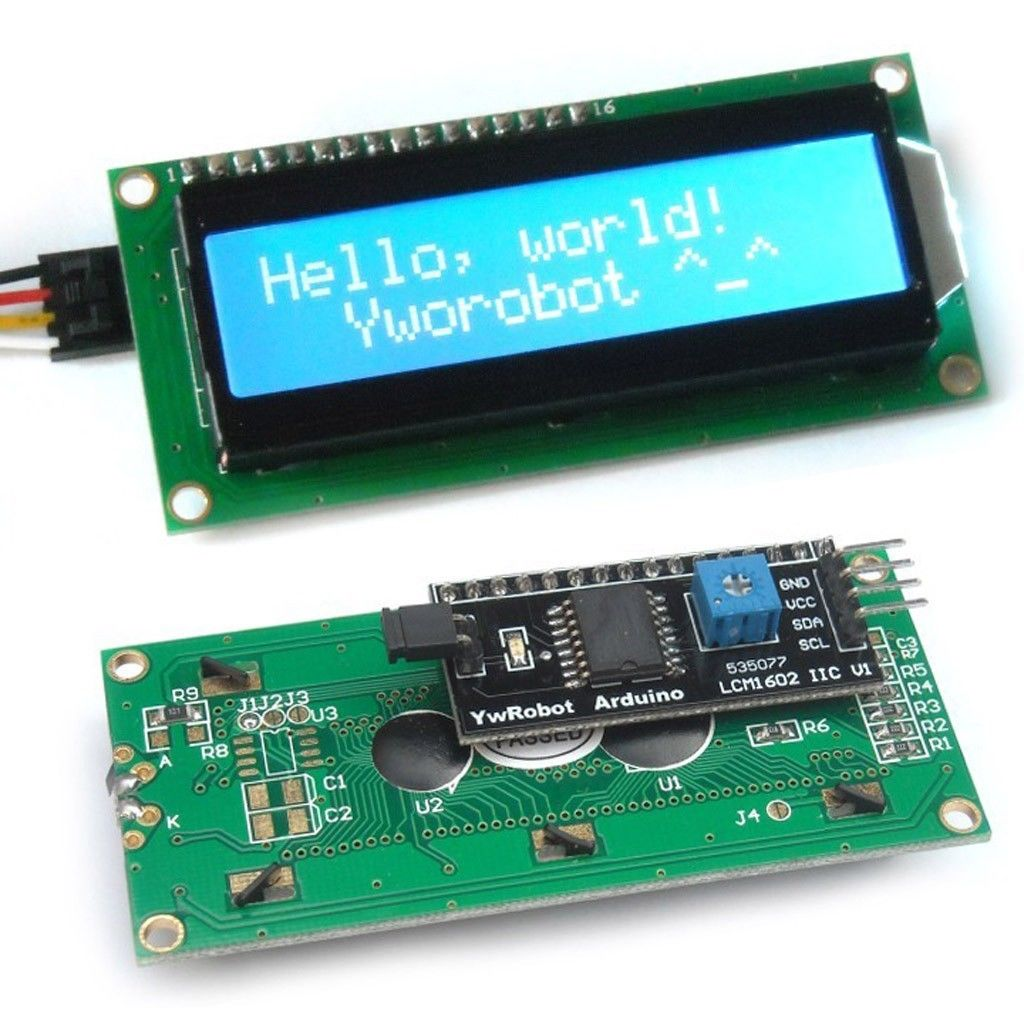
\includegraphics[width=0.4\textwidth]{images/Atividade07/03e04DisplayLCD.jpg}
\end{figure}

\begin{figure}[!ht]
  \centering
  \caption{\label{fig:05Schematic}Diagrama Esquemático desenvolvido para o Raspberry Pi B+ durante a Atividade~\ref{cha:7-placa_raspberry_pi}.}
  \fonte{Produzido pelos autores.}
  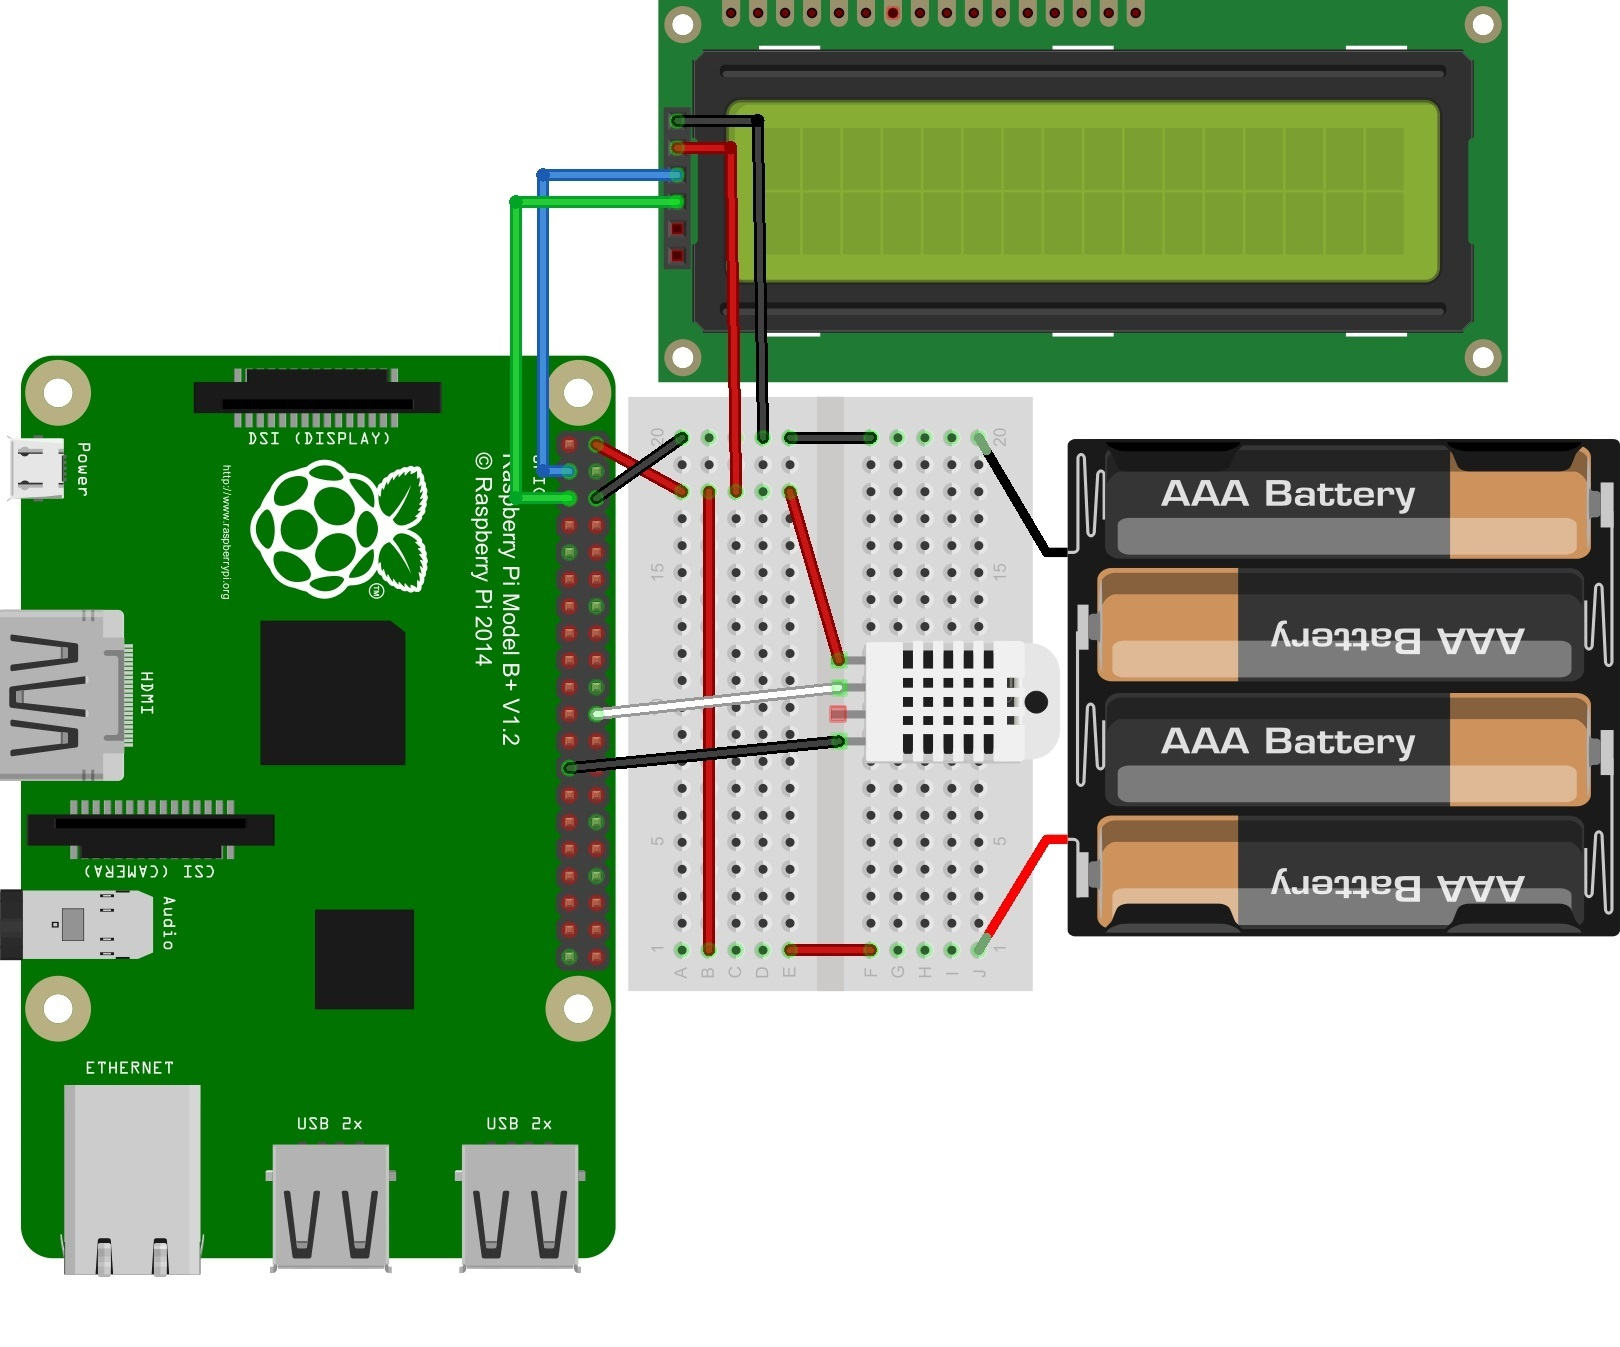
\includegraphics[width=0.5\textwidth]{images/Atividade07/05Schematic.jpg}
\end{figure}

\newpage
%inserindo algumas páginas: 1 até 7, depois 50 e 57
\begin{figure}[H]
  \centering
  \caption{\label{fig:cha-7-diagrama-pinout}Diagrama Pinout da Placa Raspberry Pi B+}
  \includepdf[pages=20,width=0.95\textwidth,frame=true,pagecommand={}]{datasheets/A4-A7-02Datasheet-introducing-the-raspberry-pi-model-b-plus-plus-differences-vs-model-b.pdf}
\end{figure}

\newpage

\begin{figure}[ht]
  \centering
  \caption{\label{fig:cha-7-idle}Programação da placa Raspberry Pi B+ no ambiente de programação IDLE do Python 3.}
  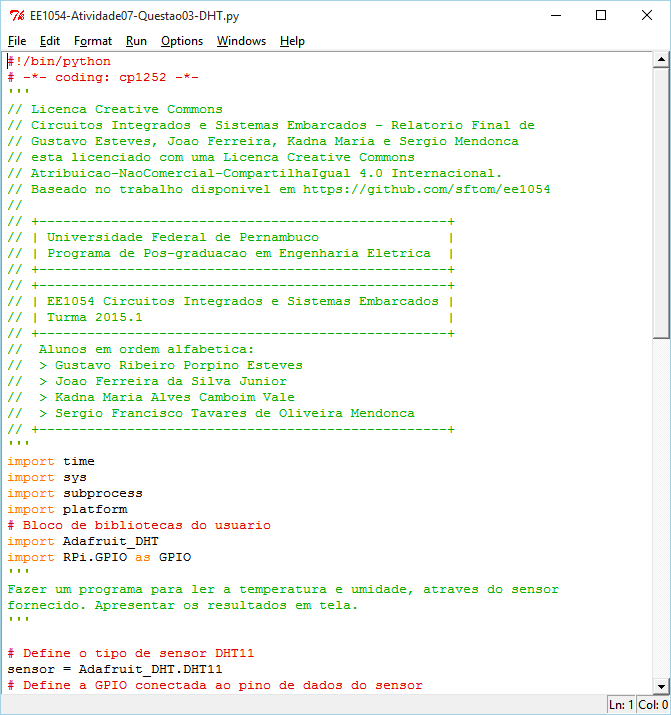
\includegraphics[width=0.8\textwidth]{images/Atividade07/IDLE.png}
\end{figure}


\newpage
Os códigos-fontes elaborados estão disponibilizados a seguir:
% ----------------------------------------------------------
\section*{Placa Raspberry Pi -- A07 (Códigos-fontes)}
\label{sec:RaspberryPi-A07Q02}
% ----------------------------------------------------------
\subsection*{A07Q02}
\lstinputlisting{sources/EE1054-Atividade07-Questao02-Print.py}


% ----------------------------------------------------------
\subsection*{A07Q03}
\lstinputlisting{sources/EE1054-Atividade07-Questao03-DHT.py}


\subsection*{A07Q04}
\lstinputlisting{sources/EE1054-Atividade07-Questao04-Display.py}


% section considerações_finais (end)

% chapter placa_raspberry_pi (end)



\chapter{Placa Intel Galileo 2nd Gen.} % (fold)
\label{cha:Placa-Intel-Galileu}

\section{Atividades propostas} % (fold)
\label{sec:RPlaca-Intel-Galileu-atividades_propostas}

\subsection*{Relatório de experimentos – Aula prática com a placa Intel Galileo}

\subsubsection*{Atividade 8}

\begin{enumerate}
  \item Instalar a ferramenta (IDE) para trabalhar com a placa Galileo e Android.
  \item Realizar testes para piscar LEDs com a placa Galileo, utilizando o LED da própria placa.
  \item Fazer um programa para gerar pulsos em um pino de saída, bem como acender um indicador (LED) ao mesmo tempo, utilizando o Shield Arduíno. Utilizar duas teclas externas uma para aumentar a velocidade das piscadas do LED e a outra para diminuir a velocidade das piscadas do LED. Pede-se o controle de velocidade de 1 a 60 piscadas.
\end{enumerate}

\section{Relatório da Atividade} % (fold)
\label{sec:consideracoes-Placa-Intel-Galileu}

Para fonte de consulta, inserimos o Diagrama de conexões da Placa Intel Galileo, como pode ser observado na Figura~\ref{fig:cha-8-diagrama-conexoes-placa-galileo}, extraída do Guia do Usuário da Placa Intel Galileo 2nd Gen. \cite{Corporation2014}.

\begin{figure}[ht]
  \centering
  \caption{\label{fig:IntelGalileo}Atividade prática na Plataforma de Desenvolvimento Intel Galileo}
  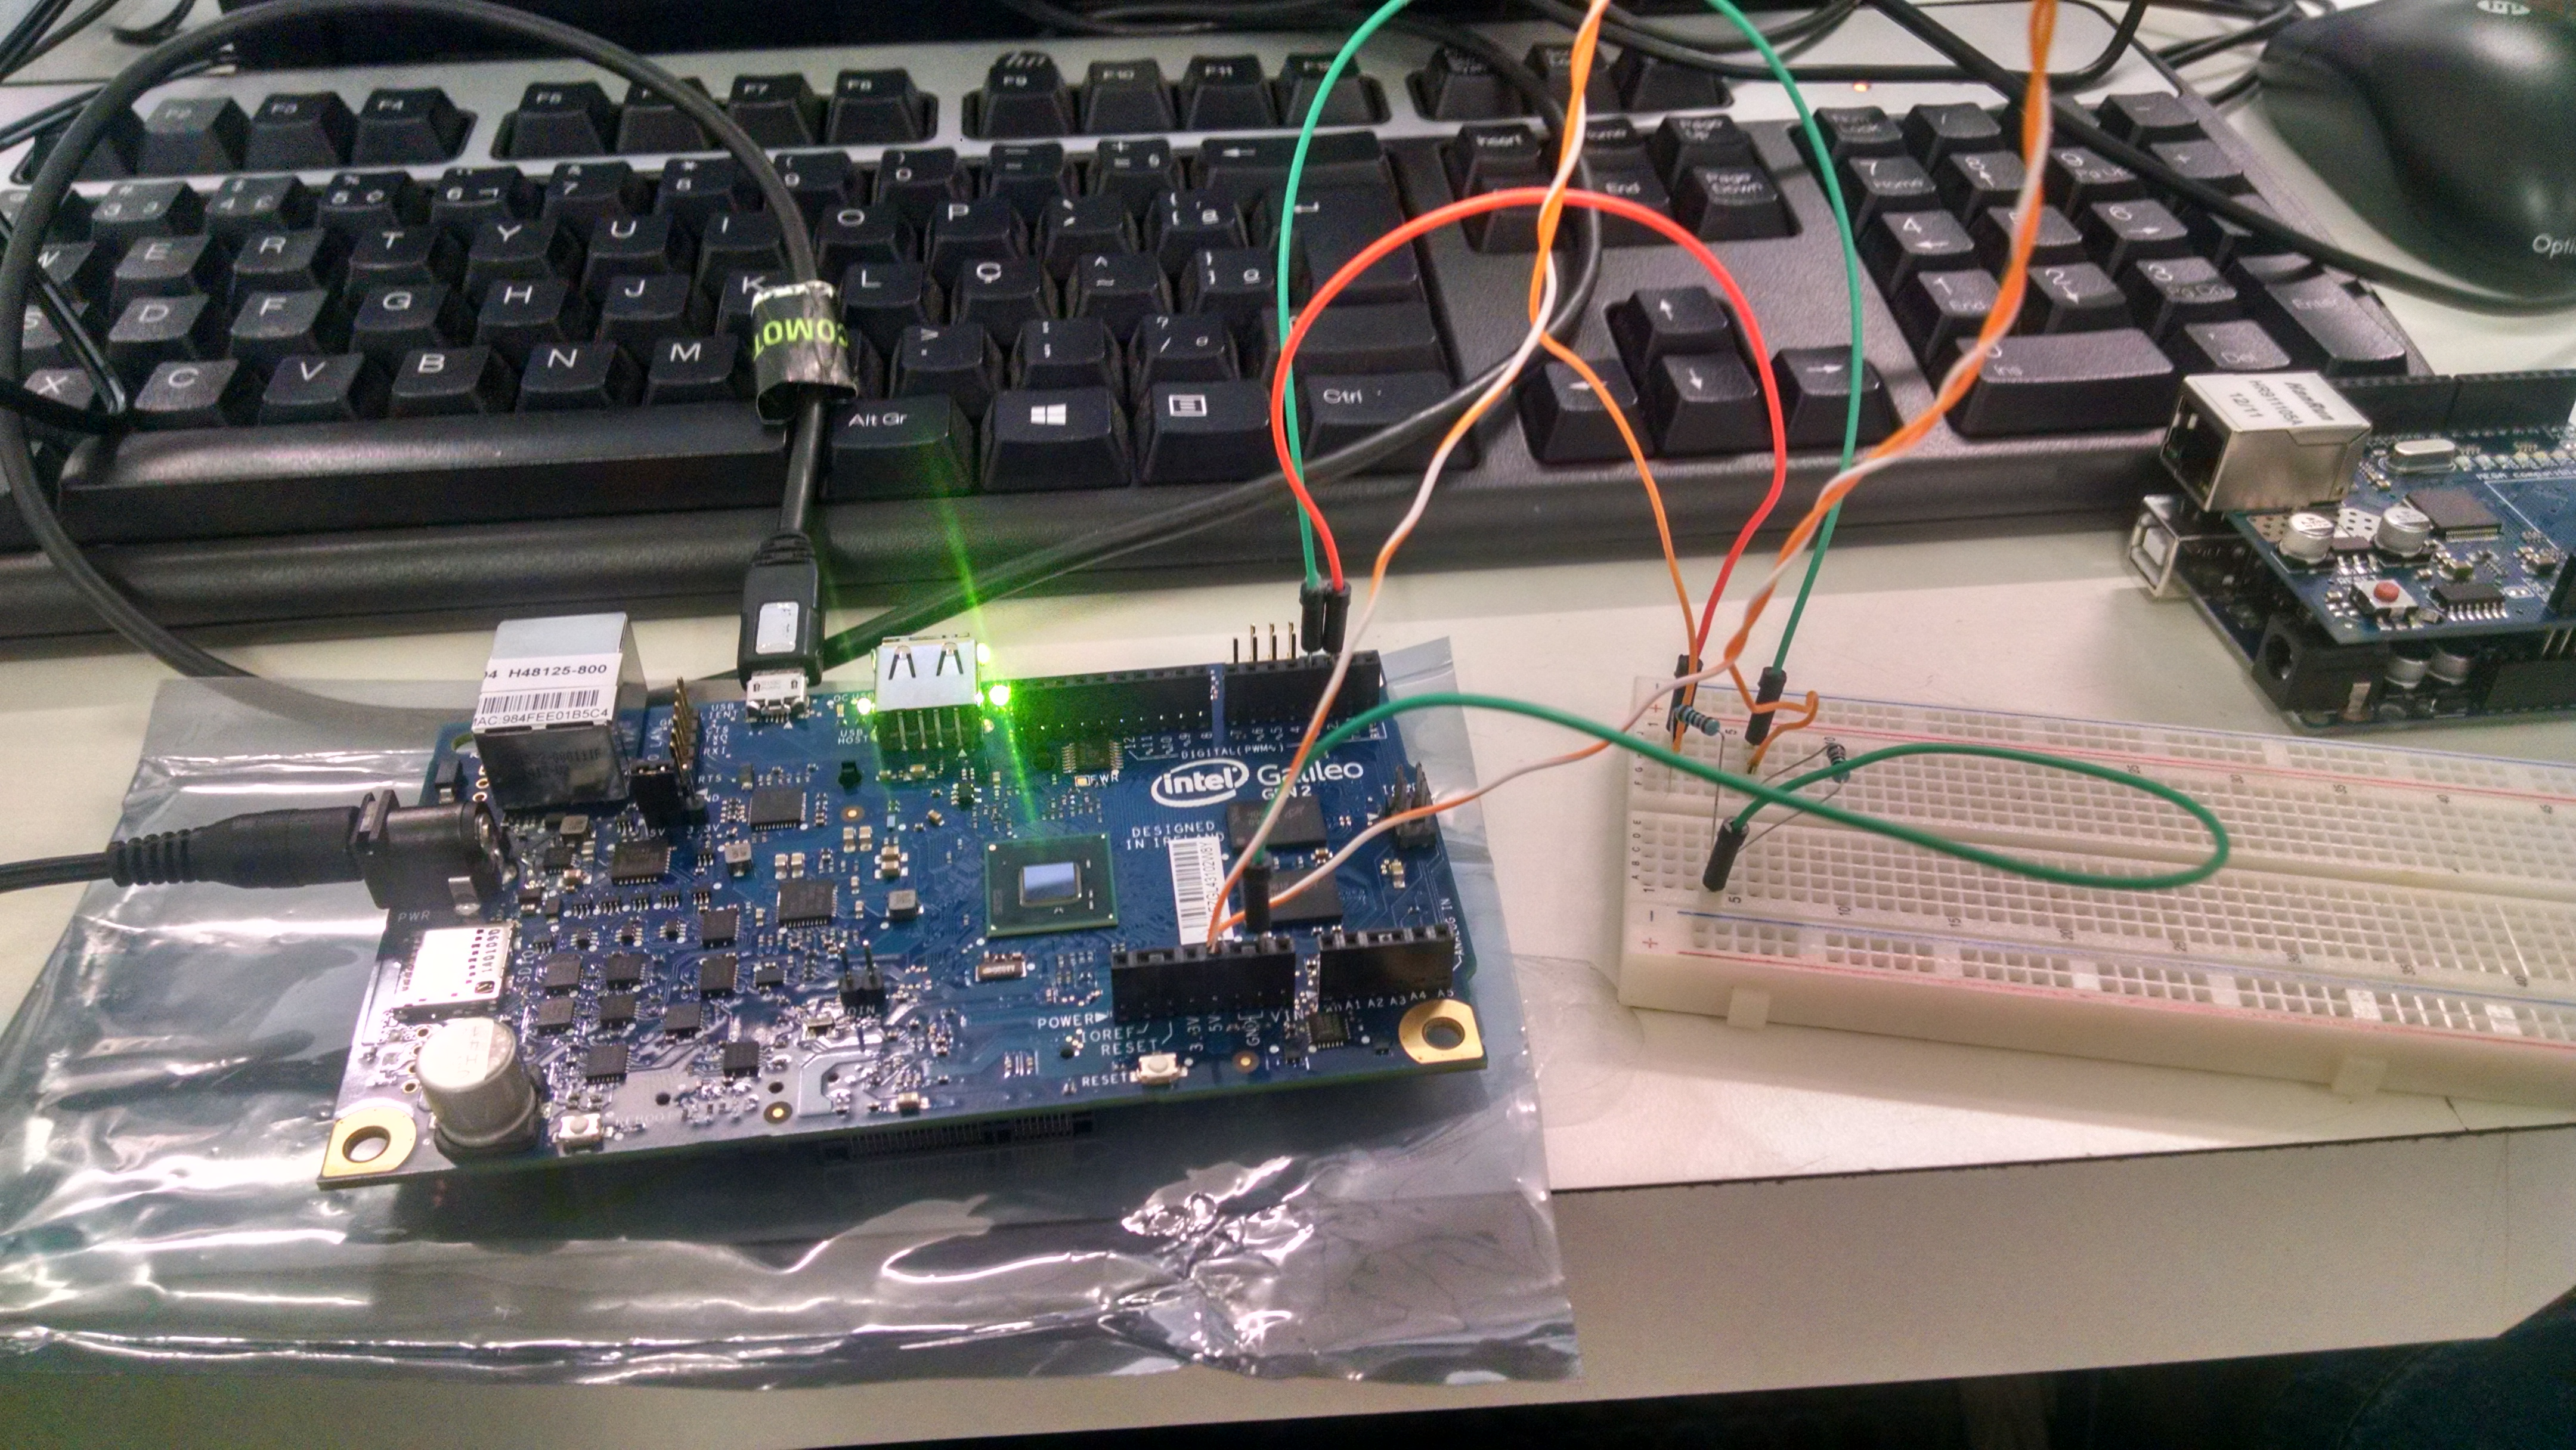
\includegraphics[width=0.8\textwidth]{images/Atividade08/IMG_20150721_145053115_HDR.jpg}
\end{figure}

\begin{figure}[ht]
  \centering
  \caption{\label{fig:05GalileoSchematic}Diagrama Esquemático desenvolvido para o Intel Galileo durante a Atividade~\ref{cha:Placa-Intel-Galileu}.}
  \fonte{Produzido pelos autores.}
  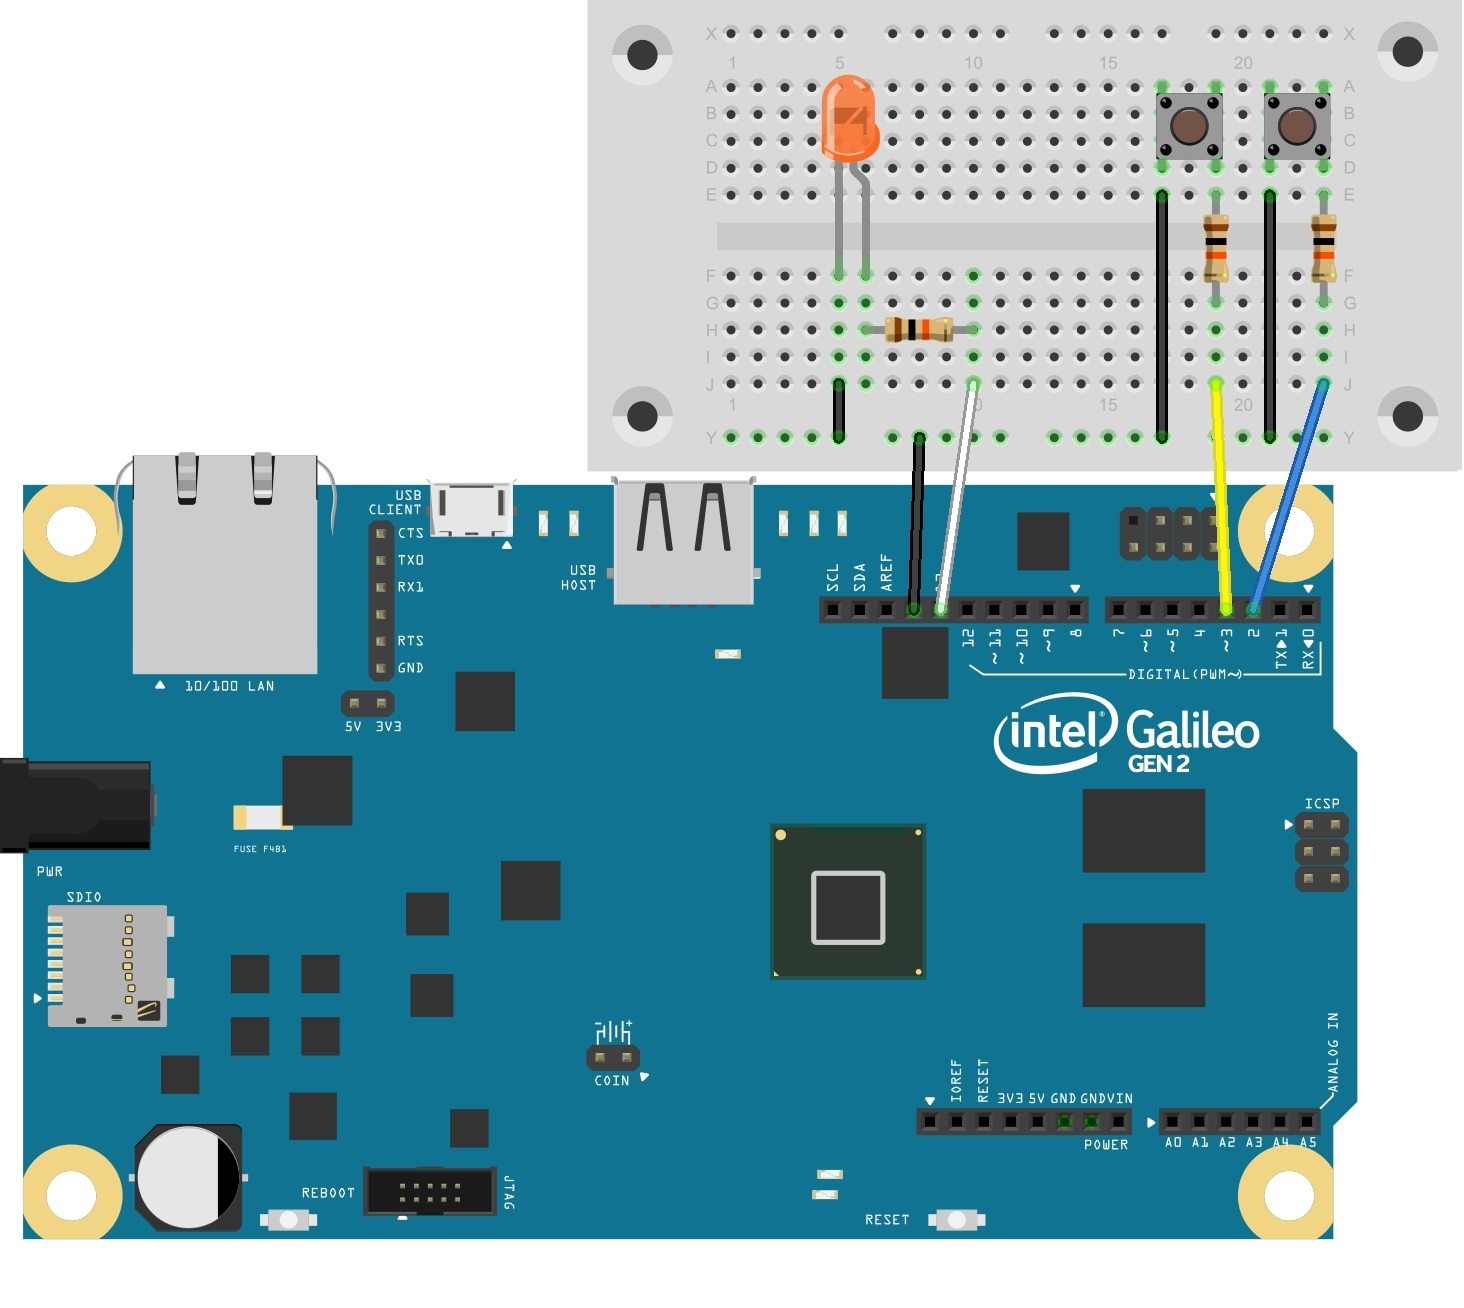
\includegraphics[width=0.8\textwidth]{images/Atividade08/05Schematic.jpg}
\end{figure}

\newpage
%inserindo algumas páginas: 1 até 7, depois 50 e 57
\begin{figure}[H]
  \centering
  \caption{\label{fig:cha-8-diagrama-conexoes-placa-galileo}Diagrama de conexões da Placa Intel Galileo.} 
  \includepdf[pages=9,width=0.95\textwidth,frame=true,pagecommand={}]{datasheets/A4-A8-02Datasheet-Galileo-BoardUserGuide-330237-001.pdf} 
\end{figure}

\newpage

\begin{figure}[ht]
  \centering
  \caption{\label{fig:cha-8-IDE-GALILEO-GEN2}Programação da placa Intel Galileo 2nd Gen. através da IDE do Arduino.}
  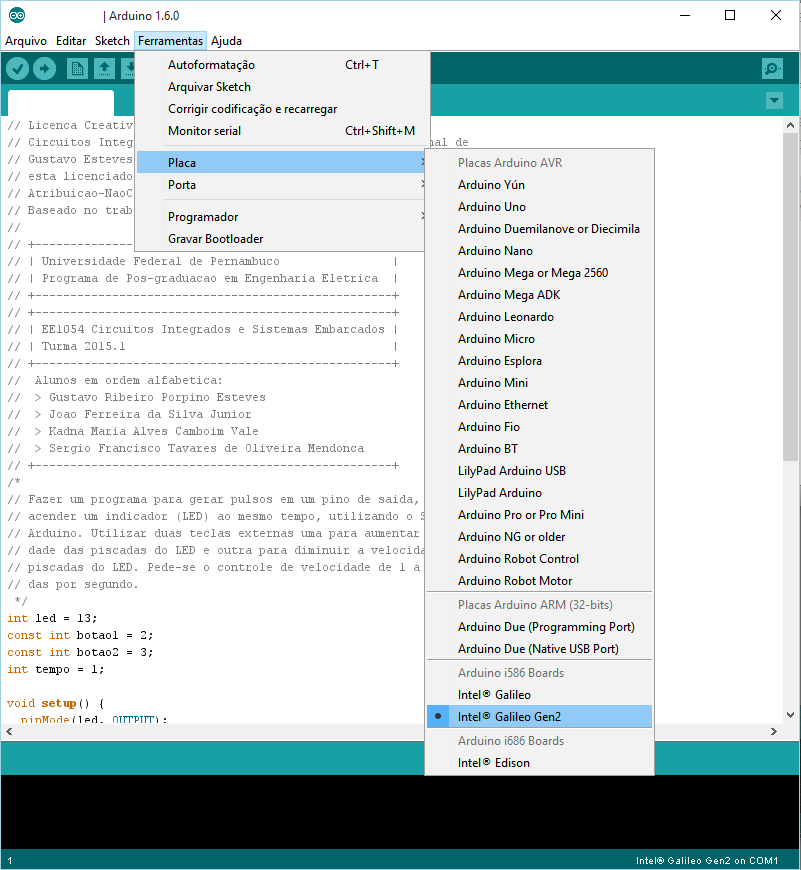
\includegraphics[width=0.8\textwidth]{images/Atividade08/IDE-GALILEO-GEN2.png}
\end{figure}


\newpage
Os códigos-fontes elaborados estão disponibilizados a seguir:
% ----------------------------------------------------------
\section*{Placa Intel Galileo -- A08 (Códigos-fontes)}
\label{sec:IntelGalileo}
% ----------------------------------------------------------
\subsection*{A08Q02-03}
\lstinputlisting{sources/EE1054-Atividade08-BlinkGalileo.ino}


% section considerações (end)

% chapter placa_intel_galileo (end)




% ----------------------------------------------------------
% Finaliza a parte no bookmark do PDF
% para que se inicie o bookmark na raiz
% e adiciona espaço de parte no Sumário
% ----------------------------------------------------------
\phantompart

% ----------------------------------------------------------
% ELEMENTOS PÓS-TEXTUAIS
% ----------------------------------------------------------
\postextual
% ----------------------------------------------------------

% ----------------------------------------------------------
% Referências bibliográficas
% ----------------------------------------------------------
\bibliography{library}
%\chapter*[Referências]{Referências}
%\addcontentsline{toc}{chapter}{Referências}


% ----------------------------------------------------------
% Glossário
% ----------------------------------------------------------
%
% Consulte o manual da classe abntex2 para orientações sobre o glossário.
%
%\glossary

% ----------------------------------------------------------
% Apêndices
% ----------------------------------------------------------

% ---
% Inicia os apêndices
% ---
% \begin{apendicesenv}

% % Imprime uma página indicando o início dos apêndices
% \partapendices

% % ----------------------------------------------------------
% \chapter{Microcontrolador ATMEL AT89S51 -- A02Q01 (códigos-fontes)}

% \section{A02Q01 (códigos-fontes)}
% \label{apendice:atmel-AT89S51}
% % ----------------------------------------------------------


% \lstinputlisting{sources/EE1054-Atividade02.c}


% % ----------------------------------------------------------
% \chapter{Microcontrolador PIC -- A03Q02 (códigos-fontes)}
% \label{apendice:PIC-A03Q02}
% % ----------------------------------------------------------
% \section*{Atividade 3, Questão 2}




% \lstinputlisting{sources/EE1054-Atividade03-Questao02-Led.c}

% % ----------------------------------------------------------
% \chapter{Microcontrolador PIC -- A03Q03 (códigos-fontes)}
% \label{apendice:PIC-A03Q03}
% % ----------------------------------------------------------
% \section*{Atividade 3, Questão 3}

% \lstinputlisting{sources/EE1054-Atividade03-Questao03-Leds-Sequencial.c}



% % ----------------------------------------------------------
% \chapter{Microcontrolador MSP430 -- A04Q02 (códigos-fontes)}
% \label{apendice:MSP430-A04Q02}
% % ----------------------------------------------------------
% \section*{Atividade 4, Questão 2}

% \lstinputlisting{sources/EE1054-Atividade04-Questao02-Led.c}


% % ----------------------------------------------------------
% \chapter{Microcontrolador MSP430 -- A04Q03 (códigos-fontes)}
% \label{apendice:MSP430-A04Q03}
% % ----------------------------------------------------------
% \section*{Atividade 4, Questão 3}

% \lstinputlisting{sources/EE1054-Atividade04-Questao03-Led-Combinacao.c}

% % ----------------------------------------------------------
% \chapter{Microcontrolador MSP430 -- A04Q04 (códigos-fontes)}
% \label{apendice:MSP430-A04Q04}
% % ----------------------------------------------------------
% \section*{Atividade 4, Questão 4}

% \lstinputlisting{sources/EE1054-Atividade04-Questao04-Pulso.c}


% % ----------------------------------------------------------
% \chapter{Microcontrolador Kinetis Freescale -- A06Q01-a (códigos-fontes)}
% \label{apendice:Kinetis-Freescale-A06Q01-a}
% % ----------------------------------------------------------
% \section*{Atividade 6, Questão 1-a}

% \lstinputlisting{sources/EE1054-Atividade06-Questao01a-Led.cpp}


% % ----------------------------------------------------------
% \chapter{Microcontrolador Kinetis Freescale -- A06Q01-b (códigos-fontes)}
% \label{apendice:Kinetis-Freescale-A06Q01-b}
% % ----------------------------------------------------------
% \section*{Atividade 6, Questão 1-b}

% \lstinputlisting{sources/EE1054-Atividade06-Questao01b-Timer.cpp}


% % ----------------------------------------------------------
% \chapter{Microcontrolador Kinetis Freescale -- A06Q01-c (códigos-fontes)}
% \label{apendice:Kinetis-Freescale-A06Q01-c}
% % ----------------------------------------------------------
% \section*{Atividade 6, Questão 1-c}

% \lstinputlisting{sources/EE1054-Atividade06-Questao01c-Touch.cpp}


% % ----------------------------------------------------------
% \chapter{Placa Raspberry Pi -- A07Q02 (códigos-fontes)}
% \label{apendice:RaspberryPi-A07Q02}
% % ----------------------------------------------------------
% \section*{Atividade 7, Questão 2}

% \lstinputlisting{sources/EE1054-Atividade07-Questao02-Print.py}


% % ----------------------------------------------------------
% \chapter{Placa Raspberry Pi -- A07Q03 (códigos-fontes)}
% \label{apendice:RaspberryPi-A07Q03}
% % ----------------------------------------------------------
% \section*{Atividade 7, Questão 3}

% \lstinputlisting{sources/EE1054-Atividade07-Questao03-DHT.py}

% % ----------------------------------------------------------
% \chapter{Placa Raspberry Pi -- A07Q04 (códigos-fontes)}
% \label{apendice:RaspberryPi-A07Q04}
% % ----------------------------------------------------------
% \section*{Atividade 7, Questão 4}

% \lstinputlisting{sources/EE1054-Atividade07-Questao04-Display.py}


% \end{apendicesenv}



% ---


% ----------------------------------------------------------
% Anexos
% ----------------------------------------------------------

% ---
% Inicia os anexos
% ---
% %inserindo apenas uma página
% \includepdf[pages=16]{arquivo01.pdf}

% %inserindo algumas páginas: 1 até 7, depois 50 e 57
% \includepdf[pages={1-7,50,57}]{arquivo02.pdf}

% %inserindo uma página em branco depois da página 1
% \includepdf[pages={1,{},2-10}]{arquivo03.pdf}

% %inserindo todas as páginas
% \includepdf[pages=-]{arquivo04.pdf}

% %inserindo múltiplas páginas numa única página
% \includepdf[pages={286-291},nup=2x3]{arquivo05.pdf}

% %inserindo páginas em landscape
% \includepdf[pages=-,landscape]{arquivo06.pdf}



% \begin{anexosenv}

% % % Imprime uma página indicando o início dos anexos
% \partanexos

% % % ---
% \chapter{Data Sheet do ATMEL AT89S51}
% \label{anexo:datasheet-atmel-AT89S51}
% % % ---
% 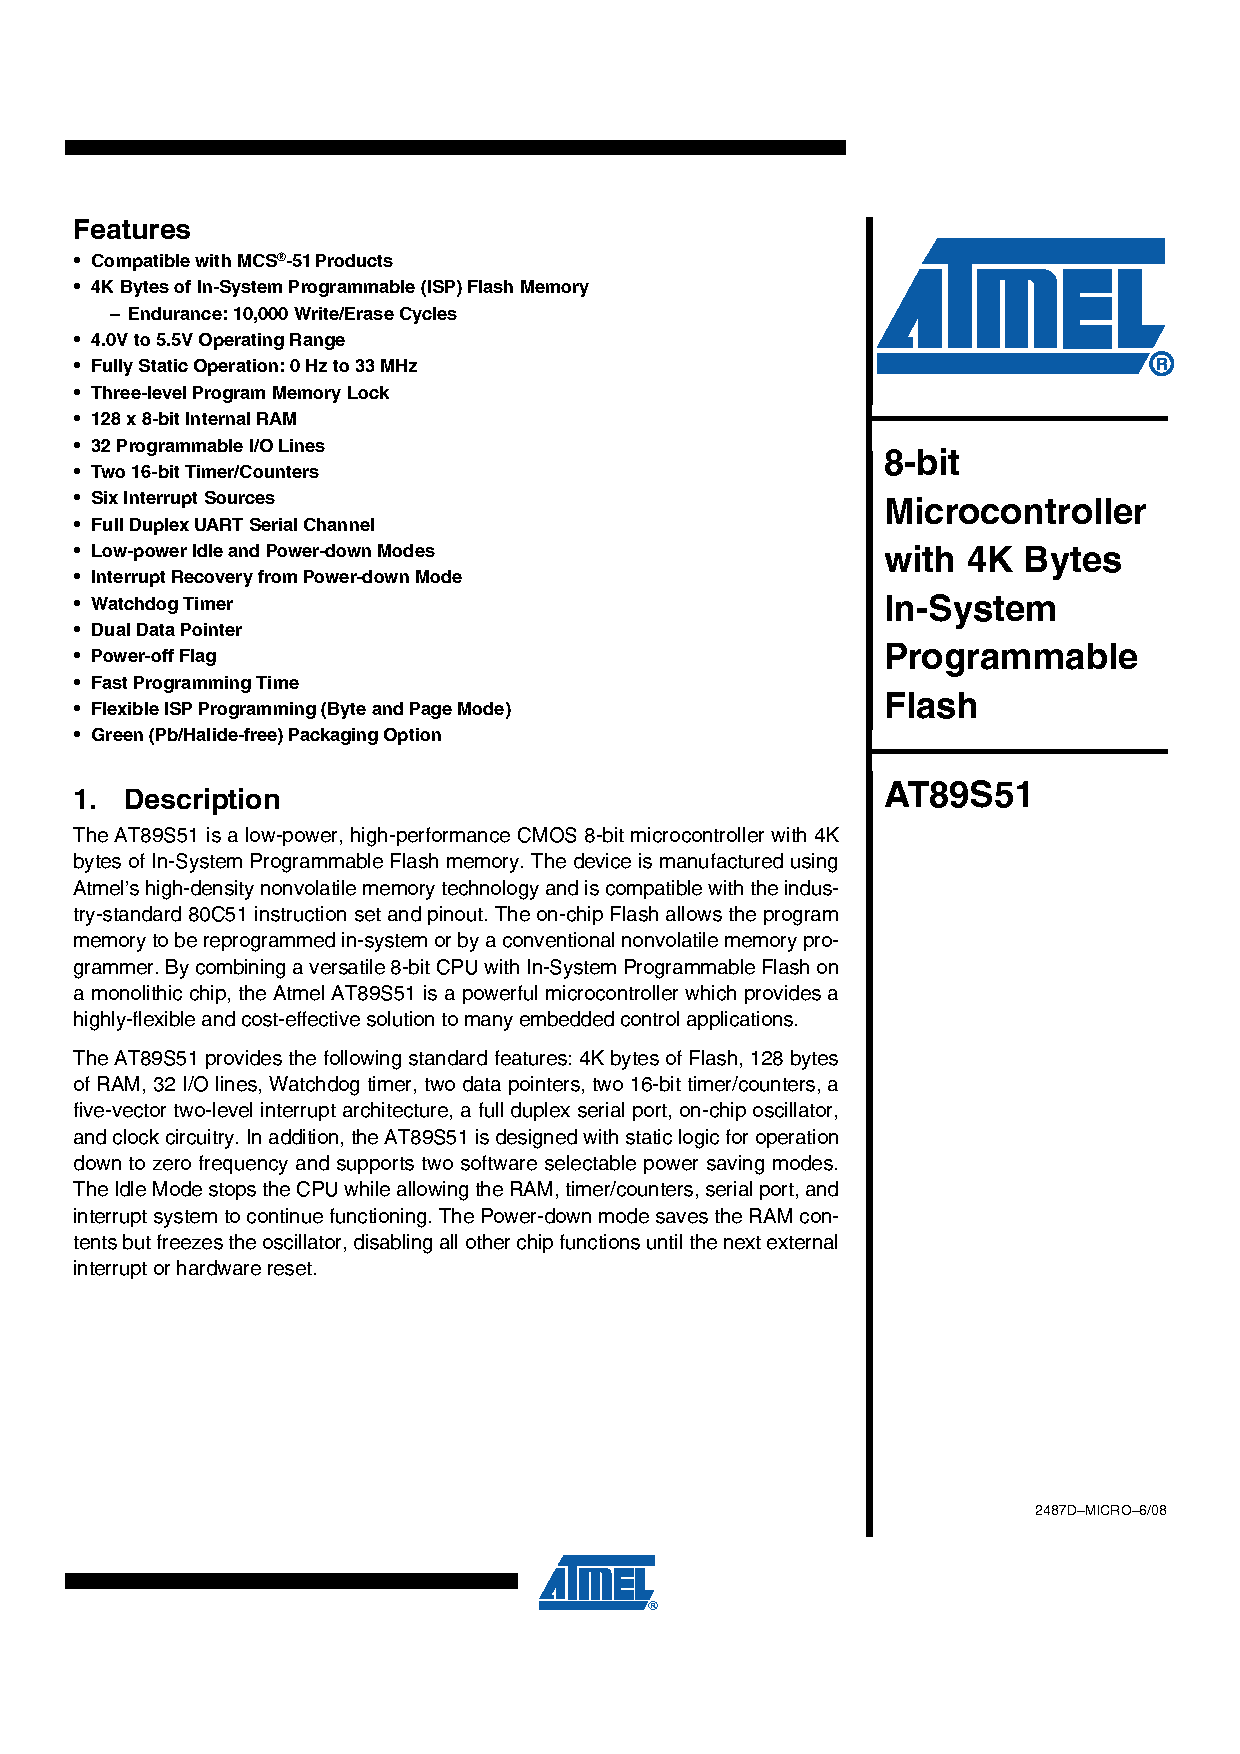
\includepdf[pages=-]{datasheets/A4-doc2487.pdf}

% % % ---
% \chapter{Data Sheet do Microship PIC}
% \label{anexo:datasheet-microship-PIC}
% % % ---
% \includepdf[pages=-]{datasheets/A4-39632e.pdf}

% % \lipsum[31]

% % % ---
% % \chapter{Fusce facilisis lacinia dui}
% % % ---

% % \lipsum[32]

% \end{anexosenv}

%---------------------------------------------------------------------
% INDICE REMISSIVO
%---------------------------------------------------------------------
% \phantompart
% \printindex
%---------------------------------------------------------------------

\end{document}